\chapter{Evaluation of the Best Classification Method}
\label{chapter_classification}
\section{Considered classification methods}
\label{sec_considered_classif}
The goal of our analysis is to classify $y \in \left\lbrace female, male \right\rbrace $ given the data matrix $\mat{X}$ of our 17 predictors. 
We are interested in determining not only the model with the best predictive performance, but also the most significant features of human voice. Therefore, we decided not to pre-process our data with a dimensionality reduction technique, such as Principal Component Analysis~(PCA). Transforming the feature space with PCA would prevent us from extracting the importance of each single predictor.
Furthermore, we argue that sensitivity and specificity are of equal importance in our setting and, thus, our objective is to minimize the total misclassification error. 
Since our classes are perfectly balanced, we use a threshold of \num{0.5} for our Bayes plug-in estimator.
In our analysis we implement the following statistical learning methods to predict the class of $ y \in \left\lbrace female, male \right\rbrace$.
\begin{itemize}
	\item \textbf{Logistic regression:} models the posterior probability of response $y\in \left\lbrace female, male \right\rbrace$, given the predictors $\mat{X}$, using the logistic function;
	
	\item \textbf{Regularized logistic regression:} Ridge~($\ell_2$) and Lasso~($\ell_1$) penalties can be used for variable shrinkage and contribute in avoiding overfitting. Especially, Lasso regularization performs variable selection and is therefore a useful approach to examine which features are significant.
	
	\item \textbf{Linear discriminant analysis (LDA):} LDA makes the assumption that the conditional densities $f \left(\mat{X}|y=male \right)$ and $ f \left(\mat{X}|y=female \right)$ are both multivariate Gaussian with a common covariance matrix. 
	It belongs to a family of techniques that use linear boundaries to separate classes in classification problems. 
	If the assumption of normality is realistic, then LDA is expected to provide better results than logistic regression;
	
	\item \textbf{Quadratic discriminant analysis (QDA):} QDA is a similar method to LDA. 
	The multivariate normality assumption remains, but unlike LDA, QDA assumes that each class has its own covariance matrix. 
	If QDA has better predictive performance than LDA, it is an indication that a linear boundary is not the optimal to separate the 2 classes.
	
	\item \textbf{k-nearest neighbors (kNN):} kNN is a non-parametric approach which is highly flexible and uses non-linear decision boundaries. 
	Before the implementation of kNN, it is crucial to scale the data since this method relies on the euclidean distance between observations;
	
	\item \textbf{Classifications trees:} Classification trees stratify the feature space recursively into simple regions and assign the label ``female'' or ``male'' using the majority vote. 
	Bagging, random forests and gradient tree boosting are also implemented with the aim of improving predictive performance;
	
	\item \textbf{Support vector machines (SVM):} SVM is also a non-parametric method that perform well in classification problems where there is a clear margin of separation. We experiment with \num{2} kernels; the linear and the radial basis function~(RBF).
\end{itemize}
For an exhaustive description of the classification methods, please refer to~\cite{ESL_2001}.
\section{Classification based on the fundamental frequency}
\label{sec_intuitive_approach}
Based on the exploratory data analysis described in Chapter~\ref{chapter_data_exploration}, we propose to perform the classification based on the ``meanfun'' feature alone. 
This will give a baseline for further analysis described in the remaining of this Chapter.

To perform the analysis, we randomly split the dataset into a training set~( \SI{80}{\percent}) and a test set~(\SI{20}{\percent}). 
The training set is used to fit the models and for best parameter selection if needed. The parameter selection is based on \num{10}-fold cross-validation. The test set is used to compute the classification error estimate used to compare the models. The classification error considered in the study is the $0-1$ loss. 
The experiments have been performed on Python \num{3}\footnote{\url{{https://github.com/AdriBesson/Statistical_learning_course/tree/develop/project}}} with a single seed number for reproducibility of the results.
\begin{table}[htb]
	\ra{1.2}
	\caption{Classification Error Estimate of the Methods for Classification With ``meanfun'' Feature}
	\begin{center}
		\begin{tabular}{@{} c c c @{}}\toprule
			Type & Methods & \\
			\midrule
			\multirow{5}{*}{Max. Likelihood} & Logistic reg. & \num{0.0536} \\
			& Logistic reg. - Ridge & \num{0.0505}  \\
			& LDA & \textbf{\num{0.0489}} \\
			& QDA & \textbf{\num{0.0489}} \\
			\cmidrule{1-3}
			\multirow{3}{*}{Trees} & Tree & \num{0.0505} \\
			& Bagging & \num{0.0505} \\
			& XGBoost & \num{0.0505}\\
			\cmidrule{1-3}
			\multirow{2}{*}{SVM} & Linear & \num{0.0505} \\
			& Gaussian & \textbf{\num{0.0489}} \\
			\cmidrule{1-3}
			x & kNN & \num{0.0520}\\
			\bottomrule
		\end{tabular}
	\end{center}
	\label{tab_res_meanfun}
\end{table}

The results, summarized in Table~\ref{tab_res_meanfun}, show that the classification error is already very low when considering only the ``meanfun'' feature. Indeed the average classification error of the different classifiers is \num{0.0505}. Thus, ``meanfun'' is a very good feature for classification which is in accordance with the exploratory data analysis described in Chapter~\ref{chapter_data_exploration}. 

Regarding the classifiers, it can be seen that some of the ones described in Section~\ref{sec_considered_classif} are not mentioned in Table~\ref{tab_res_meanfun}. Indeed, they do not make sense when considering only one feature for classification. 
About the relative performance of the different classifiers, the results are homogeneous around the average classification error and all the classifiers, even the simplest ones, perform well.

Such a results may be justified by the very low overlap between the ``male'' and ``female'' distributions observed in Chapter~\ref{chapter_data_exploration}. Indeed, it can be noticed on Figure~\ref{fig_facet} that even a simple threshold of ``meanfun" around a value of \num{0.15} would perform relatively well. 

\section{Classification based on a $80/20$ split of the dataset}
\label{sec_naive_strat}

\subsection{Experimental settings}
To perform the analysis, we randomly split the dataset into a training set~(\SI{80}{\percent}) and a test set~(\SI{20}{\percent}). 
The training set is used to fit the models and for best parameter selection if needed. 
The test set is used to compute the classification error and to compare the models. The classification error is the $0-1$ loss. 

The models compared in the study are the ones described in Section~\ref{sec_considered_classif}. 
The errors are computed for \num{5} seed numbers in order to study the variability of the models with respect to the training/test sets and their initialization. 
The results are reported in Table~\ref{tab_res_naive} and the discussions in the remainder of this Section~\ref{sec_naive_strat} are based on the test error for the seed number~\num{1}.

\begin{table}[htb]
	\ra{1.2}
	\caption{Classification Error Estimate of the Methods for Different Seed Numbers With $80/20$ Split}
	\begin{center}
		\begin{tabular}{@{} c c c  c c c c c c @{}}\toprule
			\multirow{2}{*}{Type} & \multirow{2}{*}{Methods} &  \multicolumn{5}{c}{Seed number}
			& 	\multirow{2}{*}{Mean} & \multirow{2}{*}{Std.} \\
			& & 1 & 2 & 3 & 4 & 5 & & \\
			\midrule
			\multirow{5}{*}{Max. Lik.} & Log. reg. & \num{0.0158} & \num{0.0347} & \num{0.0315} & \num{0.0237} & \num{0.0221} & \num{0.0256} & \num{0.00760} \\
			& Log. reg. - $\ell_2$ & \num{0.0158} & \num{0.0315} & \num{0.0315} & \num{0.0189} & \num{0.0284} & \num{0.0252} & \num{0.00740}\\
			& Log. reg. - $\ell_1$ & \num{0.0315} & \num{0.0363} & \num{0.0379} & \num{0.0284} & \num{0.0300} & \num{0.0328} & \num{0.00408}\\
			& LDA & \num{0.0315} & \num{0.0410} & \num{0.0379} & \num{0.0284} & \num{0.0268} & \num{0.0331} & \num{0.00611}\\
			& QDA & \num{0.0347} & \num{0.0347} & \num{0.0347} & \num{0.0268} & \num{0.0363} & \num{0.0334} & \num{0.00377}\\
			\cmidrule{1-9}
			\multirow{5}{*}{Trees} & Tree & \num{0.0379} & \num{0.0426} & \num{0.0315} & \num{0.0284} & \num{0.0300} &  \num{0.0341} & \num{0.00596}\\
			& Pruned Tree & \num{0.0394} & \num{0.0473} & \num{0.0347} & \num{0.0363} & \num{0.0300} & \num{0.0375} & \num{0.00645}\\  
			& Bagging & \num{0.0237} & \num{0.0410} & \num{0.0142} & \textbf{\num{0.0174}} & \num{0.0284} & \num{0.0249} & \num{0.0105}\\
			& Random Forest & \num{0.0189} & \num{0.0347} & \textbf{\num{0.0126}} & \num{0.0205} & \num{0.0205} & \num{0.0215}  & \num{0.00809}\\
			& XGBoost & \num{0.0189} & \textbf{\num{0.0268}} & \textbf{\num{0.0126}} & \num{0.0205} & \textbf{\num{0.0189}} & \textbf{\num{0.0196}}  & \num{0.00506}\\
			\cmidrule{1-9}
			\multirow{2}{*}{SVM} & Linear & \textbf{\num{0.0142}} & \num{0.0315} & \num{0.0284} & \num{0.0189} & \num{0.0252} & \num{0.0237}  & \num{0.00705}\\
			& Gaussian & \num{0.0205} & \num{0.0284} & \textbf{\num{0.0126}} & \textbf{\num{0.0174}} & \num{0.0205} & \num{0.0199} & \num{0.00575}\\
			\cmidrule{1-9}
			x & kNN & \num{0.0300} & \num{0.0347} & \num{0.0252} & \num{0.0379} & \num{0.0300}& \num{0.0315}  & \num{0.00486} \\
			\bottomrule
			\end{tabular}
			\end{center}
			\label{tab_res_naive}
\end{table}

\subsection{Maximum-likelihood methods}
\paragraph{Logistic regression}
If we run logistic regression on our \num{17} features, we obtain an error rate of 0.0158. The reported p-values indicate that, at \SI{5}{\percent} significance level, the coefficients of the following features are significantly non-zero: ``Q25'', ``Q75'', ``sp.ent'', ``sfm'', ``meanfun'' and ``minfun''. We observe that the lowest p-value corresponds to ``meanfun'', which shows the importance of this particular feature in voice analysis.
\paragraph{Regularized logistic regression}
We observe that Ridge regularization gives the same results as logistic regression. However, Lasso regularization performs worse providing a test error of \num{0.0315}. Lasso shrinks the coefficients of 9 predictors to zero, letting only non-zero the following ones: ``Q25'', ``Q75'', ``skew'', ``sfm'', ``mode'', ``minfun'', ``maxfun'' and ``meanfun''. The largest coefficient corresponds to ``meanfun'', confirming its significance.
%%%%%%%%%%%% FIGURE %%%%%%%%%%%
\setlength{\BoxPlotFigWidth}{0.6\textwidth}
\settoheight{\BoxPlotFigHeight}{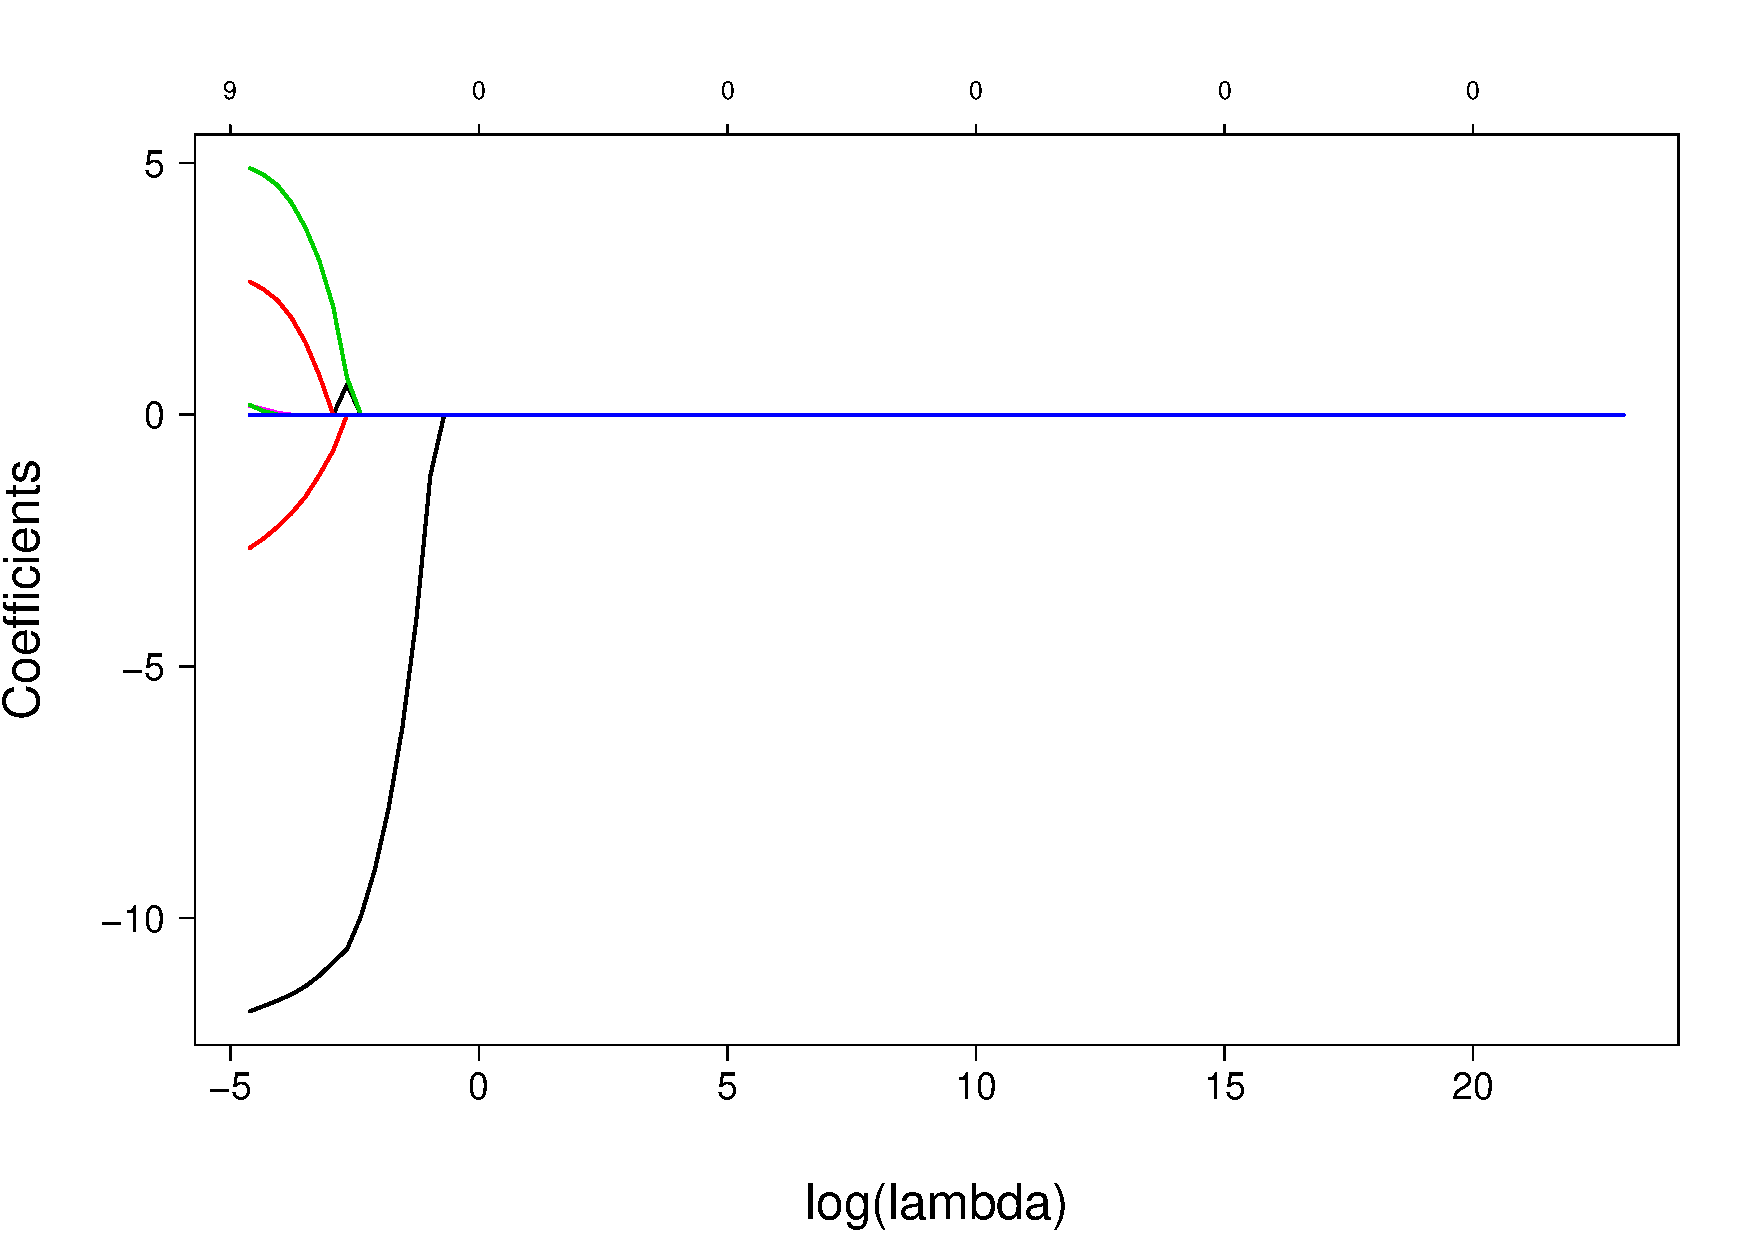
\includegraphics[width=\BoxPlotFigWidth]{figures/lasso.pdf}}
\begin{figure}[htb]
	% Maximum length
	\centering
	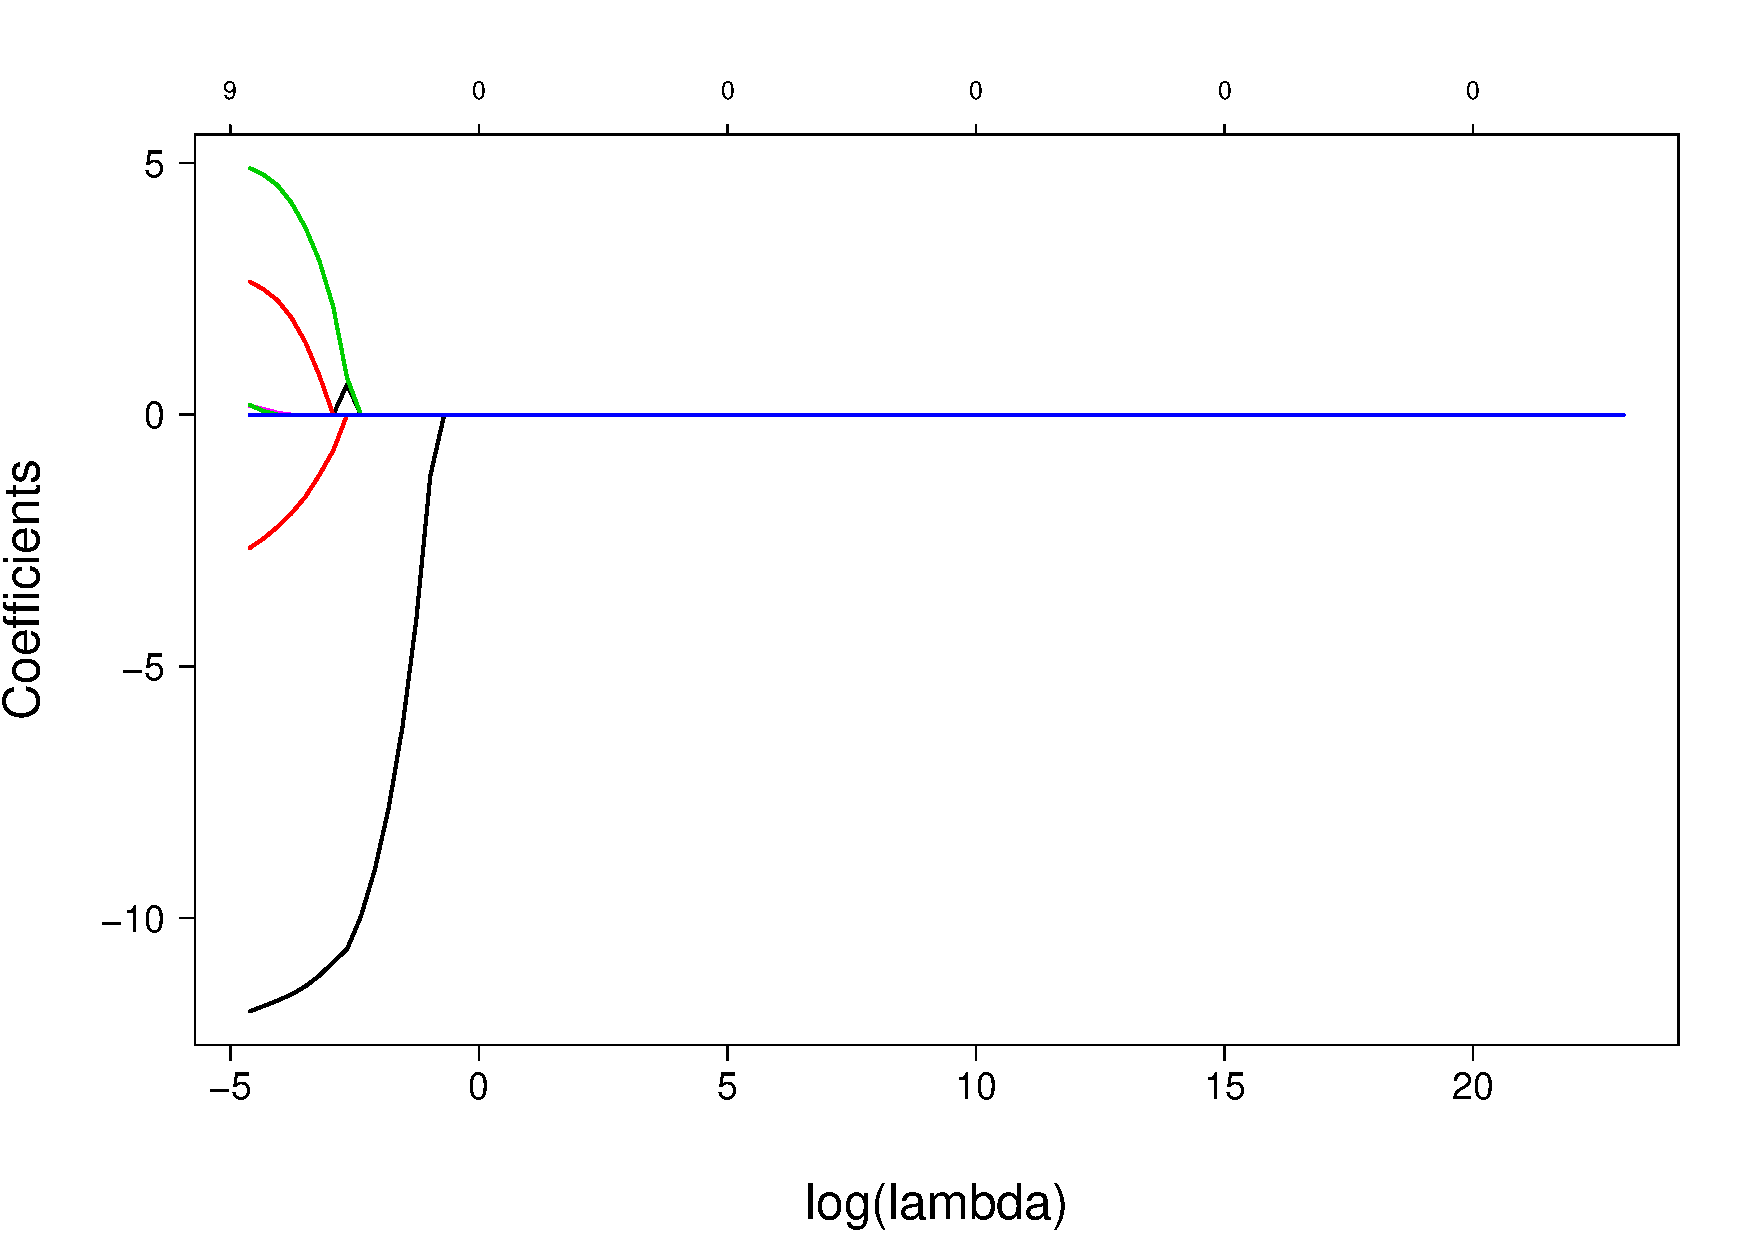
\includegraphics[height=\BoxPlotFigHeight]{figures/lasso.pdf}\hfill%
\caption{Parameters shrinkage for logistic regression with Lasso regularization.}
\label{fig_lasso_logreg}
\end{figure}
%%%%%%%%%%%% END OF FIGURE %%%%%%%%%%%
\paragraph{Linear discriminant analysis}
LDA gives a test error of \num{0.0315}. In order to check whether the model assumptions are actually satisfied, we resort to Mardia's test\footnote{\url{https://cran.r-project.org/web/packages/MVN/index.html}} for multivariate normality. Mardia's test is based on the multivariate extensions of skewness and kurtosis measures. Under the null hypothesis, our sample is drawn from a multivariate normal. 
We run Mardia's test on the two data matrices corresponding to male and female classes and conclude that normality assumption is violated. Furthermore, the two covariance matrices are not quite similar and one can argue that the assumption of a common covariance matrix is unrealistic.
To sum up, LDA seems to perform well, despite the lack of normality. We suspect that the reason lies in some particularity of our data set.
\paragraph{Quadratic discriminant analysis}
As we have mentioned above, the two covariance matrices of our two classes (male/female) are not sufficiently close. Hence we expect QDA to perform better than LDA. However, this is not the case, since QDA yields a slightly higher test error.
\subsection{k-Nearest neighbors}
We use \num{10}-fold cross validation with one-standard-error rule to find that the optimal value for parameter k, is $k=9$, as described on Figure~\ref{fig_best_param_CNN}. Then we implement \num{9}-NN, which yields a test error of \num{0.03}. We observe a slight improvement compared to LDA and QDA, which can be attributed to the high flexibility of kNN. We reckon that the linear boundary is not the most appropriate to separate the \num{2} classes.
%%%%%%%%%%%% FIGURE %%%%%%%%%%%
\settoheight{\BoxPlotFigHeight}{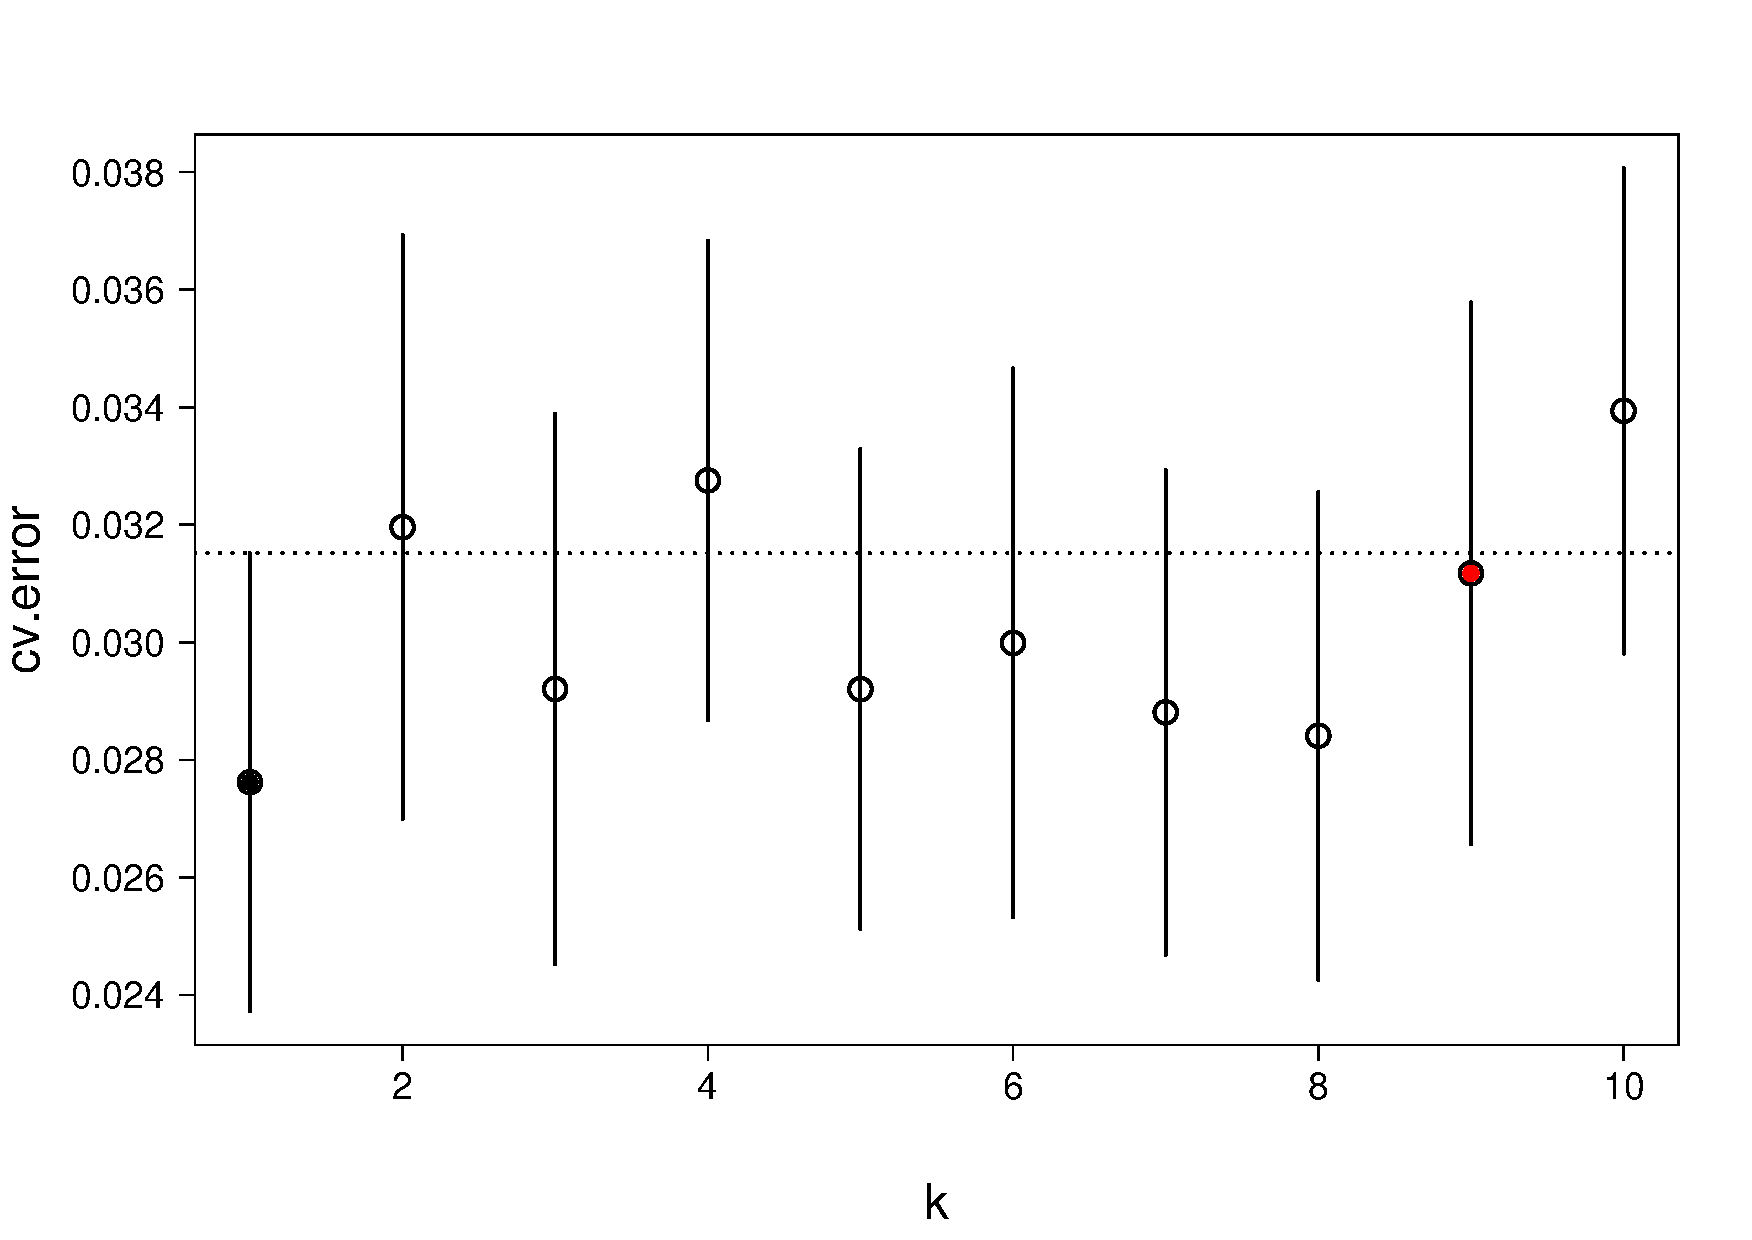
\includegraphics[width=\BoxPlotFigWidth]{figures/kNN_new.pdf}}
\begin{figure}[htb]
	% Maximum length
	\centering
	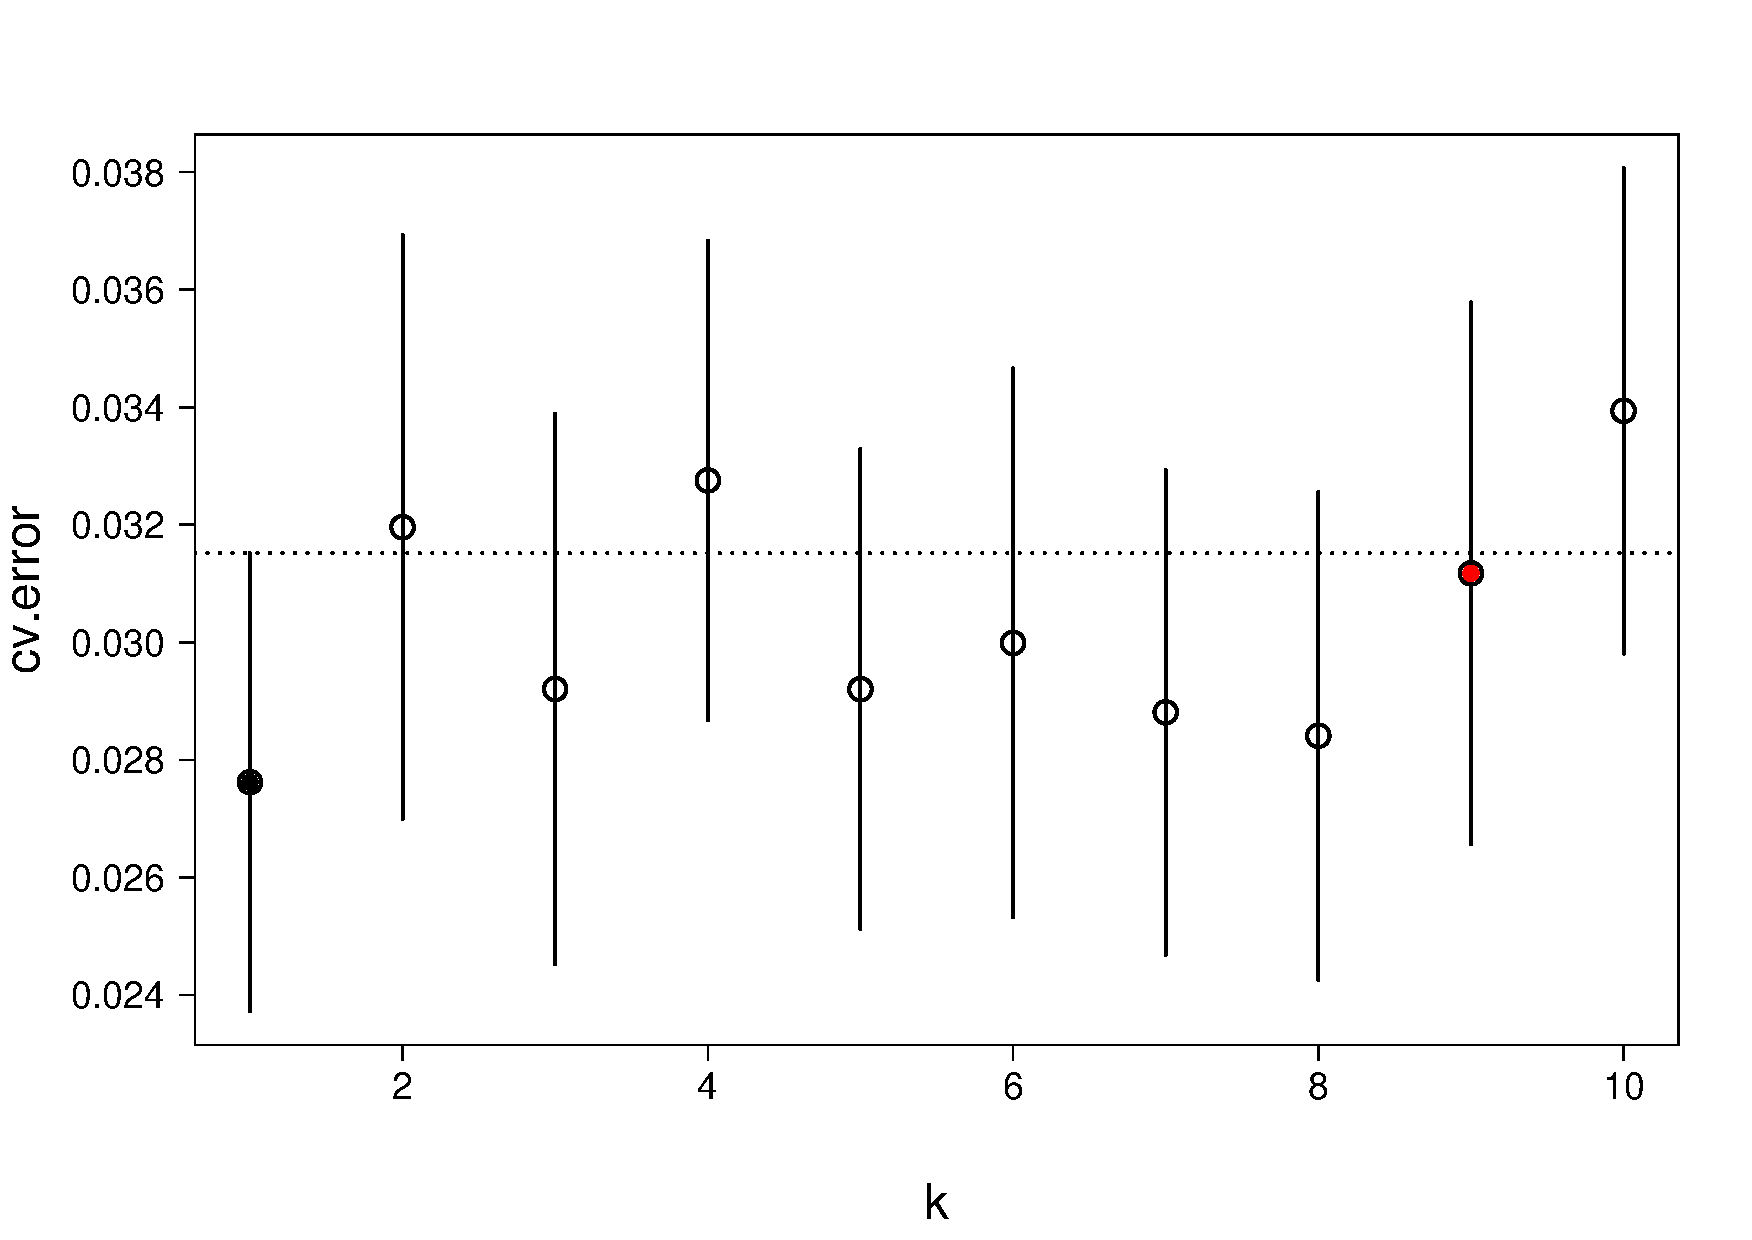
\includegraphics[height=\BoxPlotFigHeight]{figures/kNN_new.pdf}\hfill%
	\caption{Best parameter selection for kNN based on the one-standard error rule.}
	\label{fig_best_param_CNN}
\end{figure}
%%%%%%%%%%%% END OF FIGURE %%%%%%%%%%%
\subsection{Tree-based methods}
\paragraph{Classification trees}
We begin with fitting a large unpruned tree to our data. We use the cross-entropy impurity measure to grow our tree and obtain a test error of \num{0.038}. Although its predictive performance is quite good in our case, its high complexity prevents it from being interpretable as Figure~\ref{fig_tree} manifests.

After fitting a large tree, it is sensible to prune it in order to improve its interpret-ability and avoid overfitting. We prune our tree using \num{10}-fold cross validation to determine the cost-complexity parameter, and misclassification error as the loss function. Although the test error has slightly increased, the pruned tree can now be used to convey meaningful results as shown on Figure~\ref{fig_pruned_tree}. We also observe that ``meanfun'' is used in the first node, confirming, for one more time, its integral role.
%%%%%%%%%%%% FIGURE %%%%%%%%%%%
\setlength{\BoxPlotFigWidth}{0.48\textwidth}
\settoheight{\BoxPlotFigHeight}{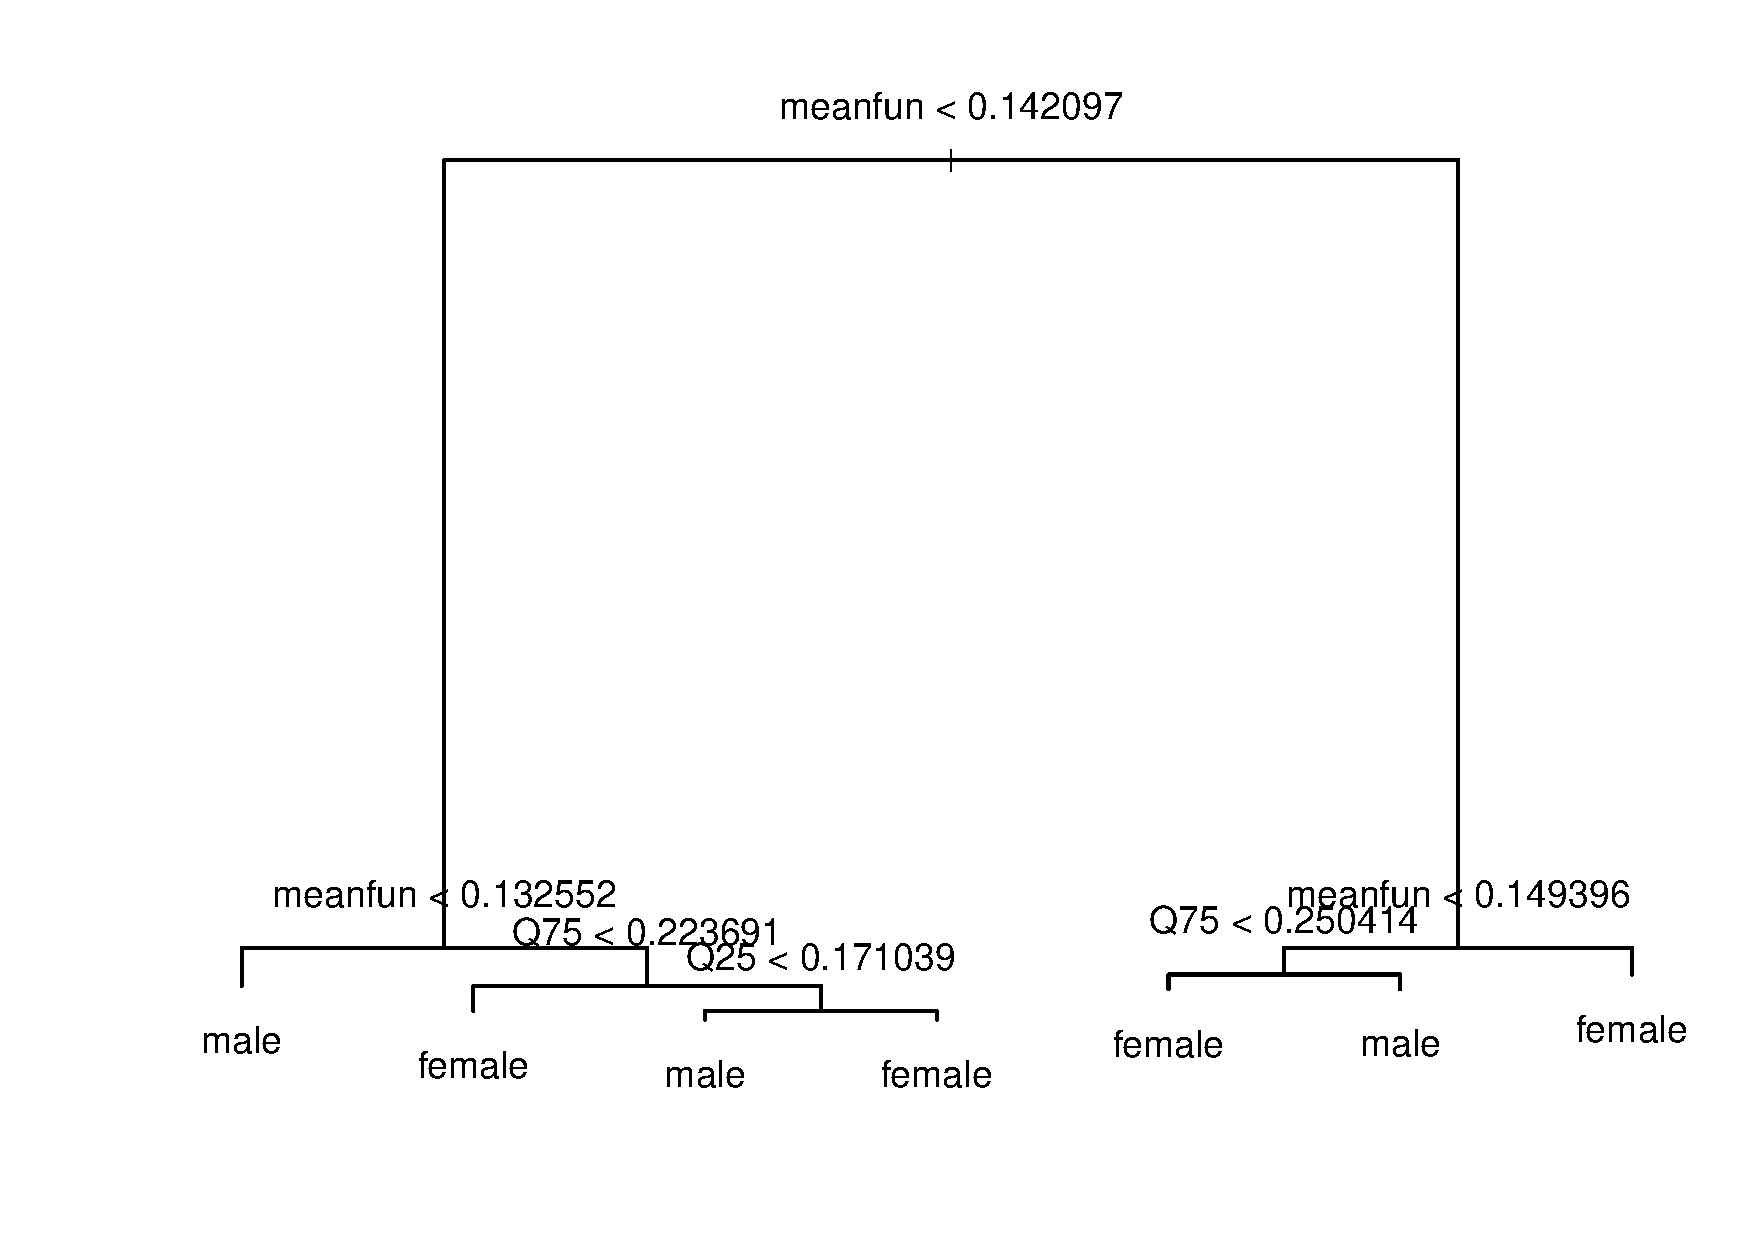
\includegraphics[width=\BoxPlotFigWidth]{figures/pruned.pdf}}
\begin{figure}[htb]
	% Maximum length
	\hfill%
	\subcaptionbox{\label{fig_tree}}{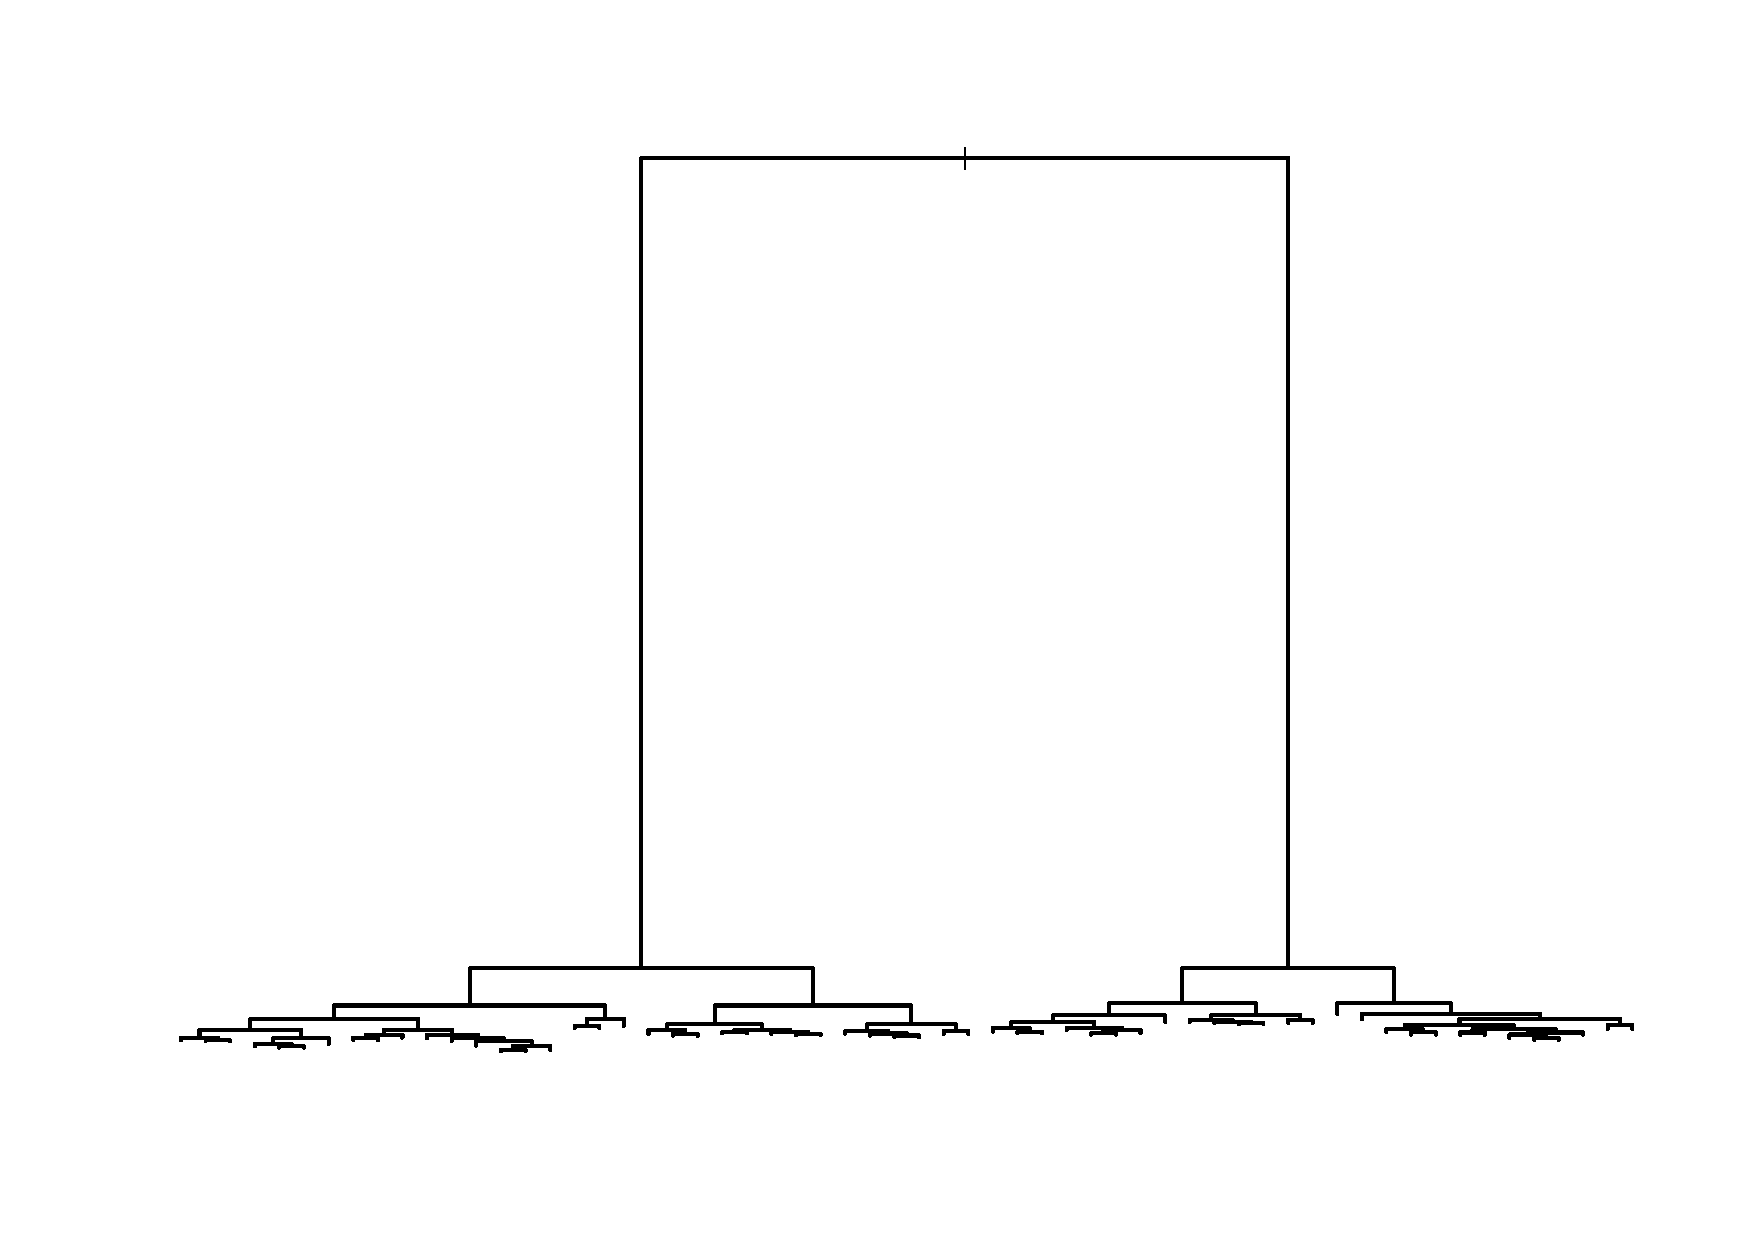
\includegraphics[height=\BoxPlotFigHeight]{figures/tree.pdf}}\hfill%
	\subcaptionbox{\label{fig_pruned_tree}}{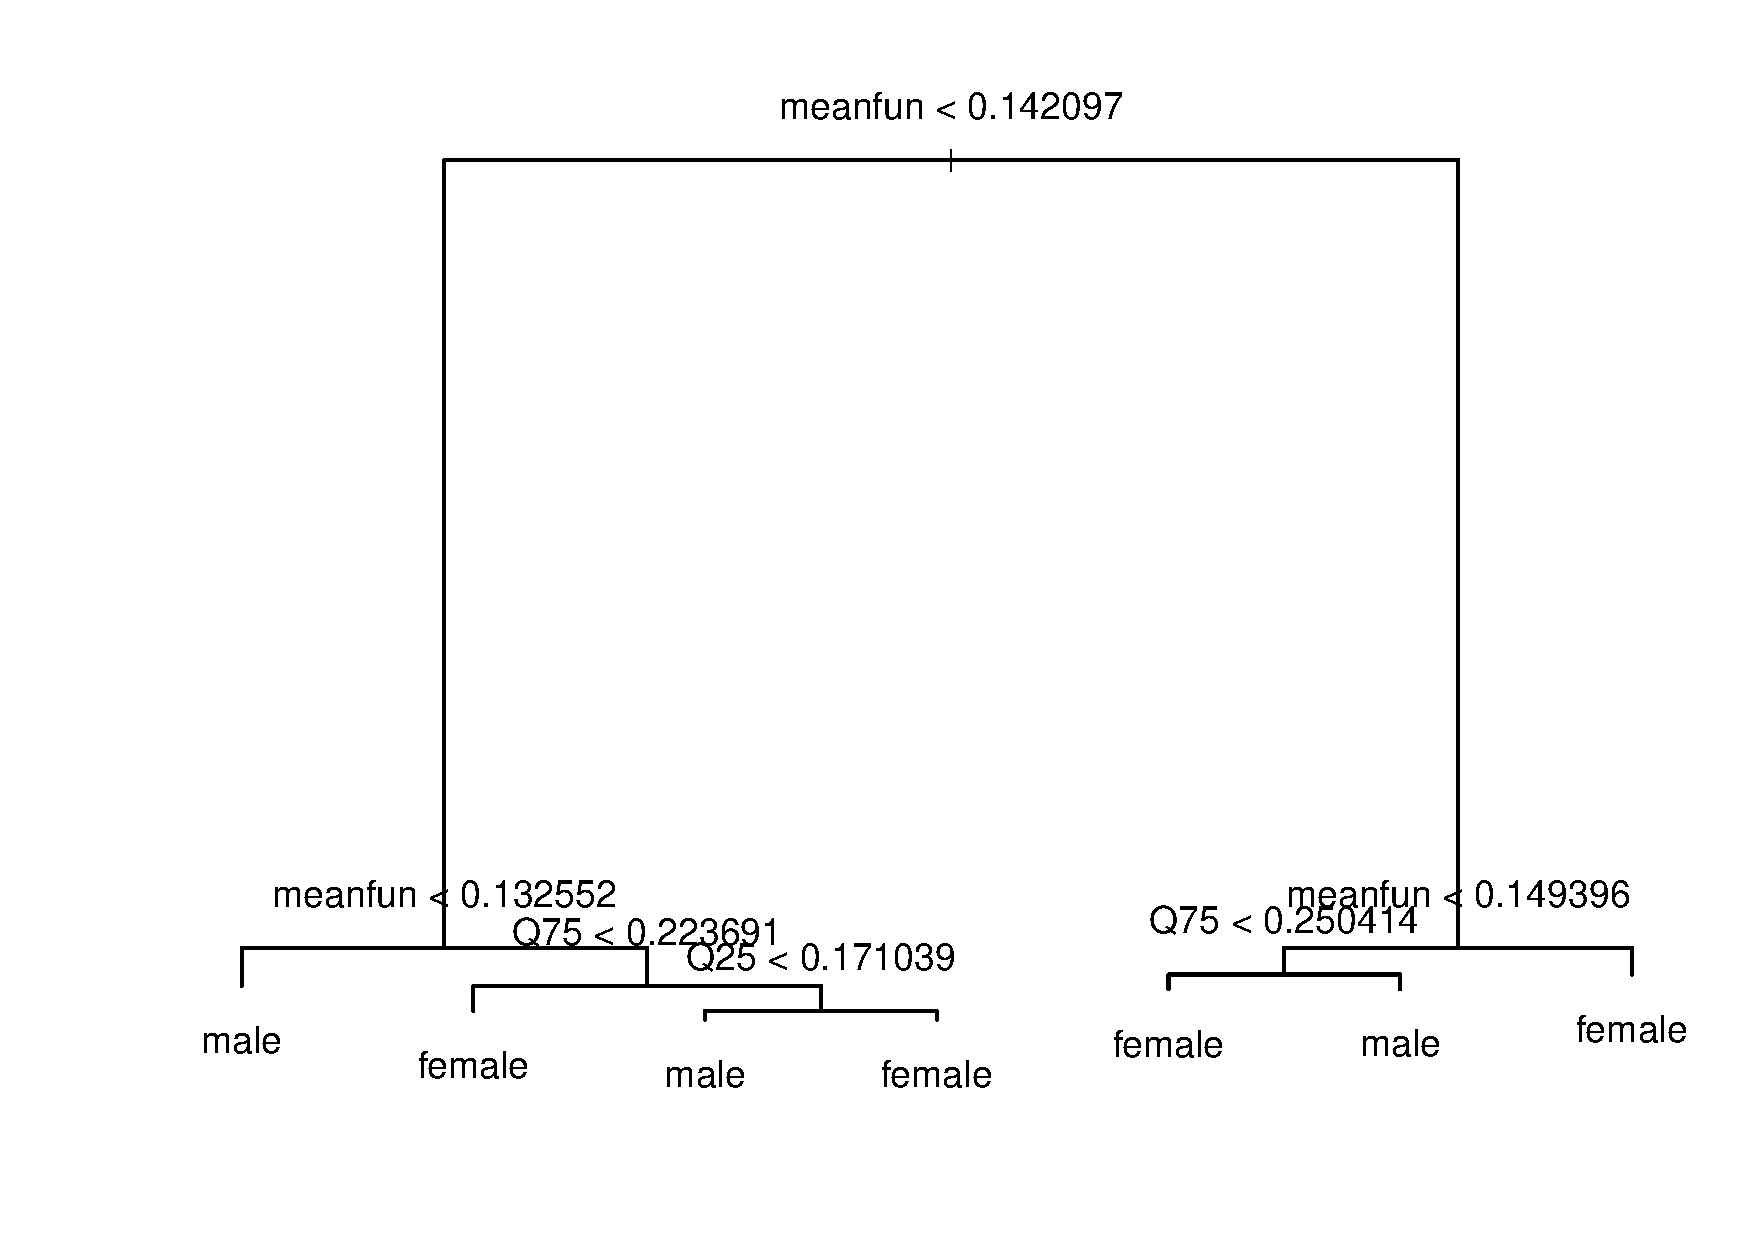
\includegraphics[height=\BoxPlotFigHeight]{figures/pruned.pdf}}\hfill\null%
	\caption{(a)- Unpruned and (b)-pruned tree.}
	\label{fig_tree}
\end{figure}
%%%%%%%%%%%% END OF FIGURE %%%%%%%%%%%
\paragraph{Bagging}
Unpruned trees have low bias but suffer from high variance. Bagging can substantially reduce the variance of unstable procedures like trees, and improve predictive performance. Bagging indeed improves accuracy of our trees, since we obtain a test error of \num{0.0237}. We also stress the importance of Out-of-Bag error estimate, which, in our case, is quite close to the test error, as it can be observed on Figure~\ref{fig_oob_bagging}.
\paragraph{Random forests}
We proceed our analysis with running a random forest. We are particularly interested in this method, since random forests provide measures of variable importance. Mean decrease accuracy and mean decrease gini metrics, the latter being displayed on Fig.~\ref{fig_feature_imp}, indicate that ``meanfun'' is the most influential feature, followed by ``Q25''. The test error is \num{0.0189}, which confirms the superb predictive performance of random forests. Again, Out-of-Bag error estimate gives an accurate estimate of test error as it can be observed on Fig.~\ref{fig_oob_rf}.
%%%%%%%%%%%% FIGURE %%%%%%%%%%%
\settoheight{\BoxPlotFigHeight}{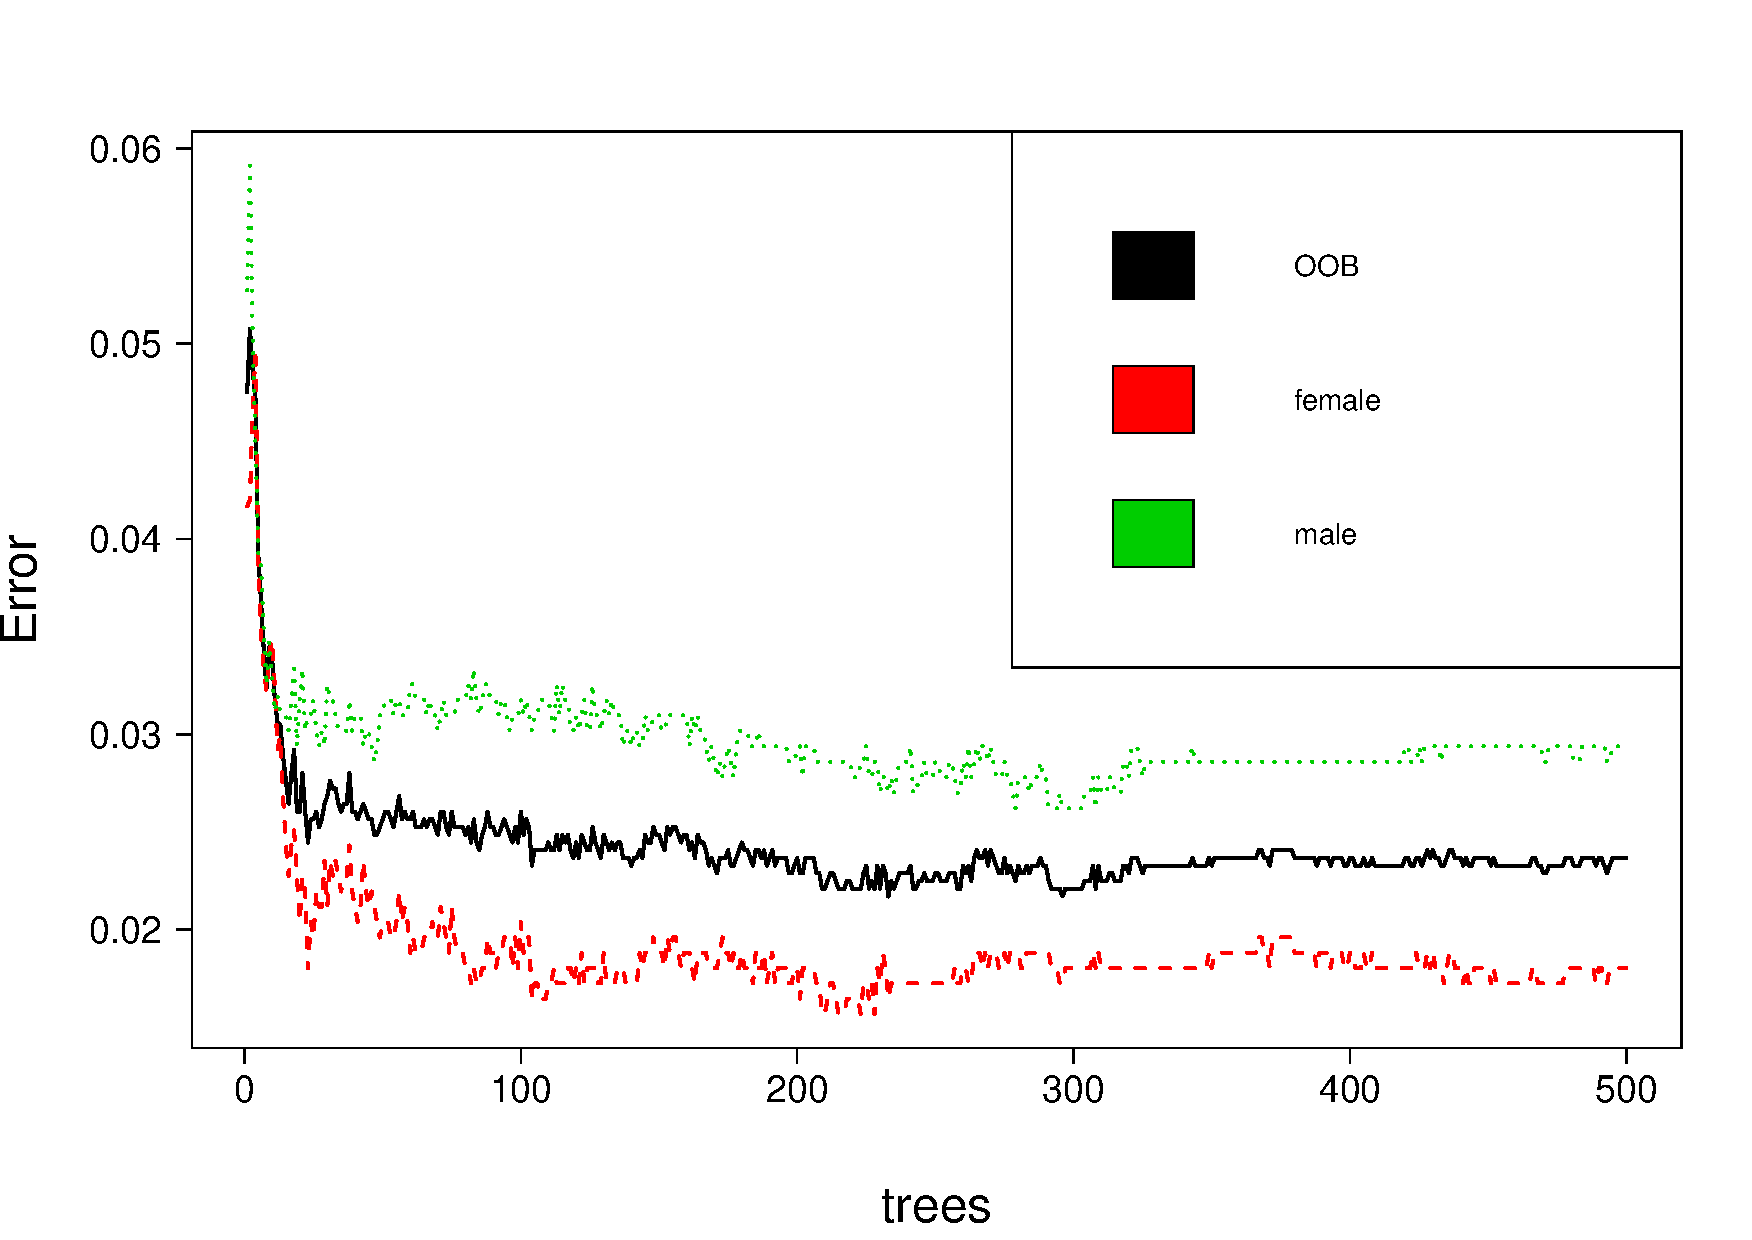
\includegraphics[width=\BoxPlotFigWidth]{figures/bagging.pdf}}
\begin{figure}[htb]
	% Maximum length
	\hfill%
	\subcaptionbox{\label{fig_oob_bagging}}{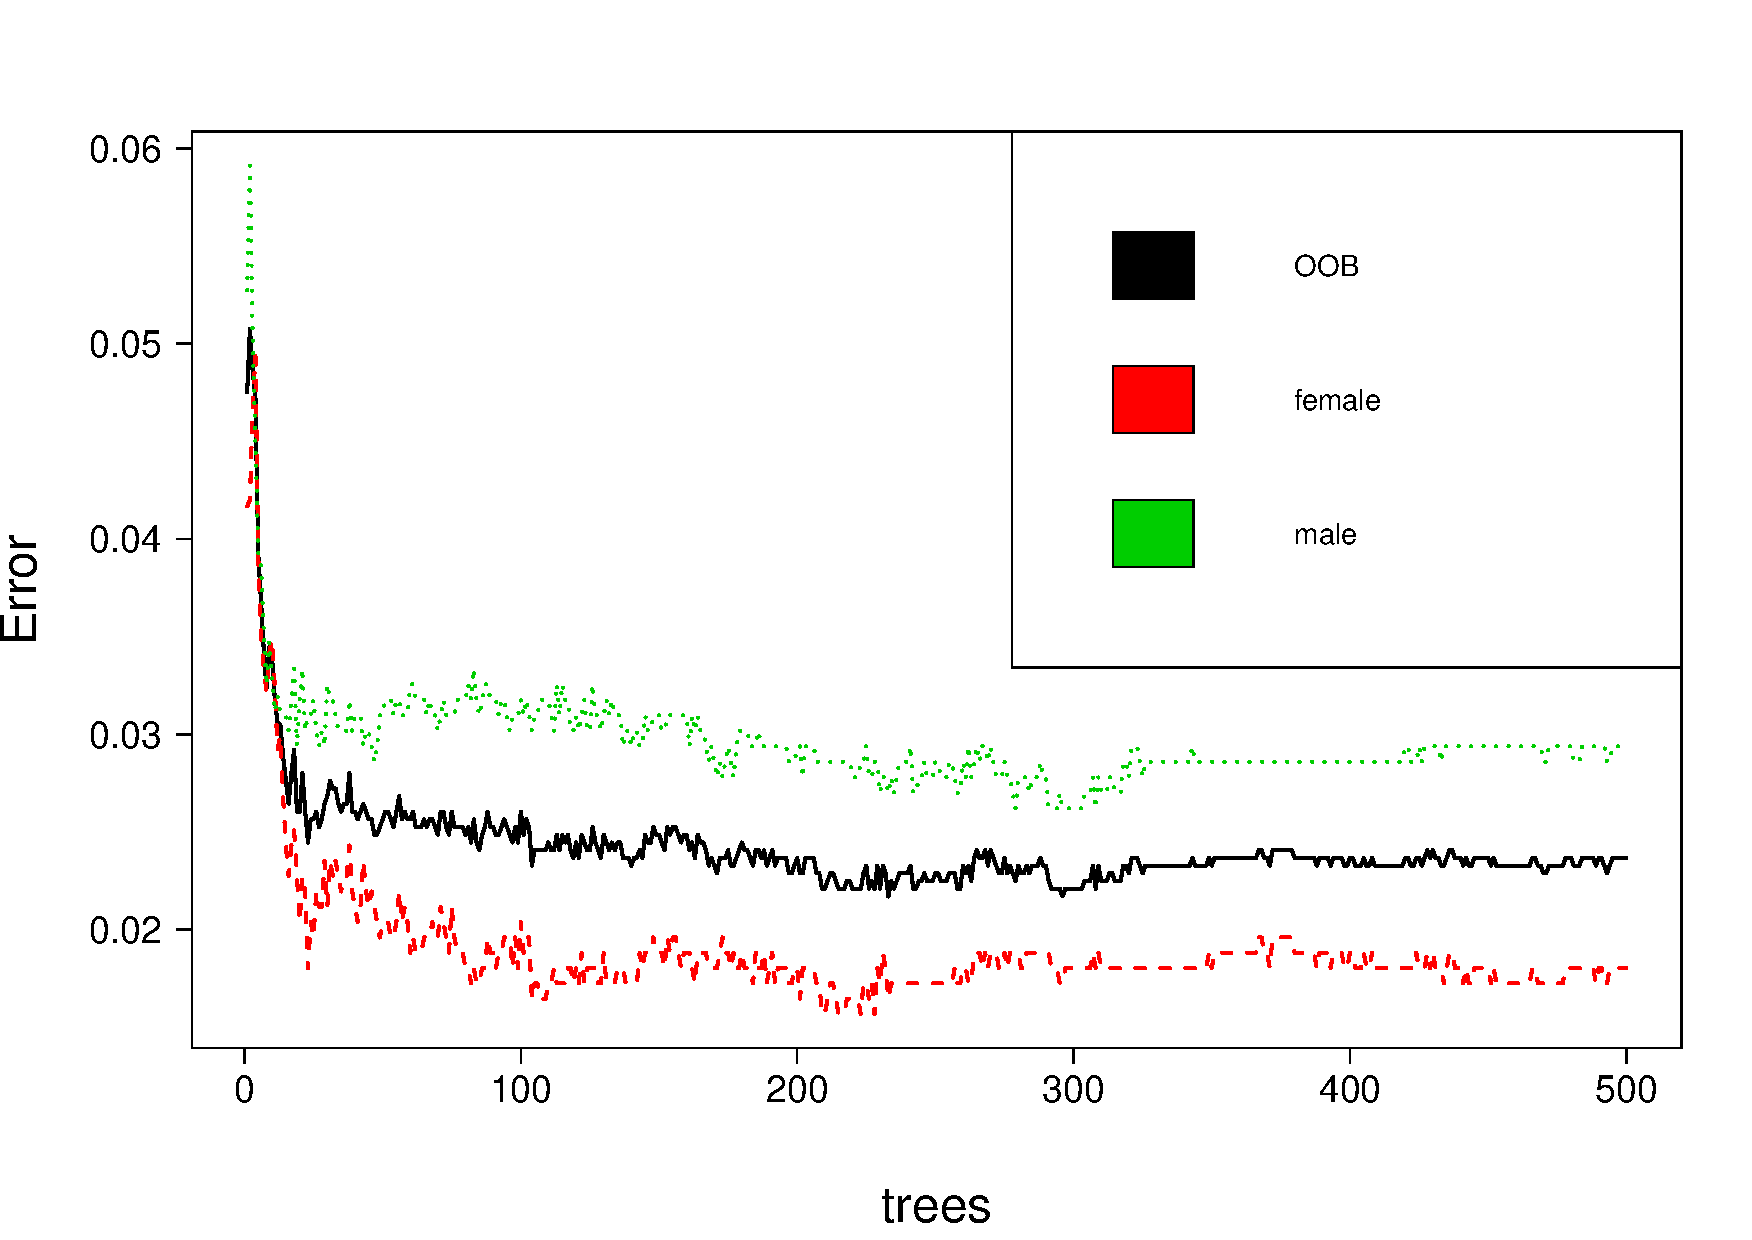
\includegraphics[height=\BoxPlotFigHeight]{figures/bagging.pdf}}\hfill%
	\subcaptionbox{\label{fig_oob_rf}}{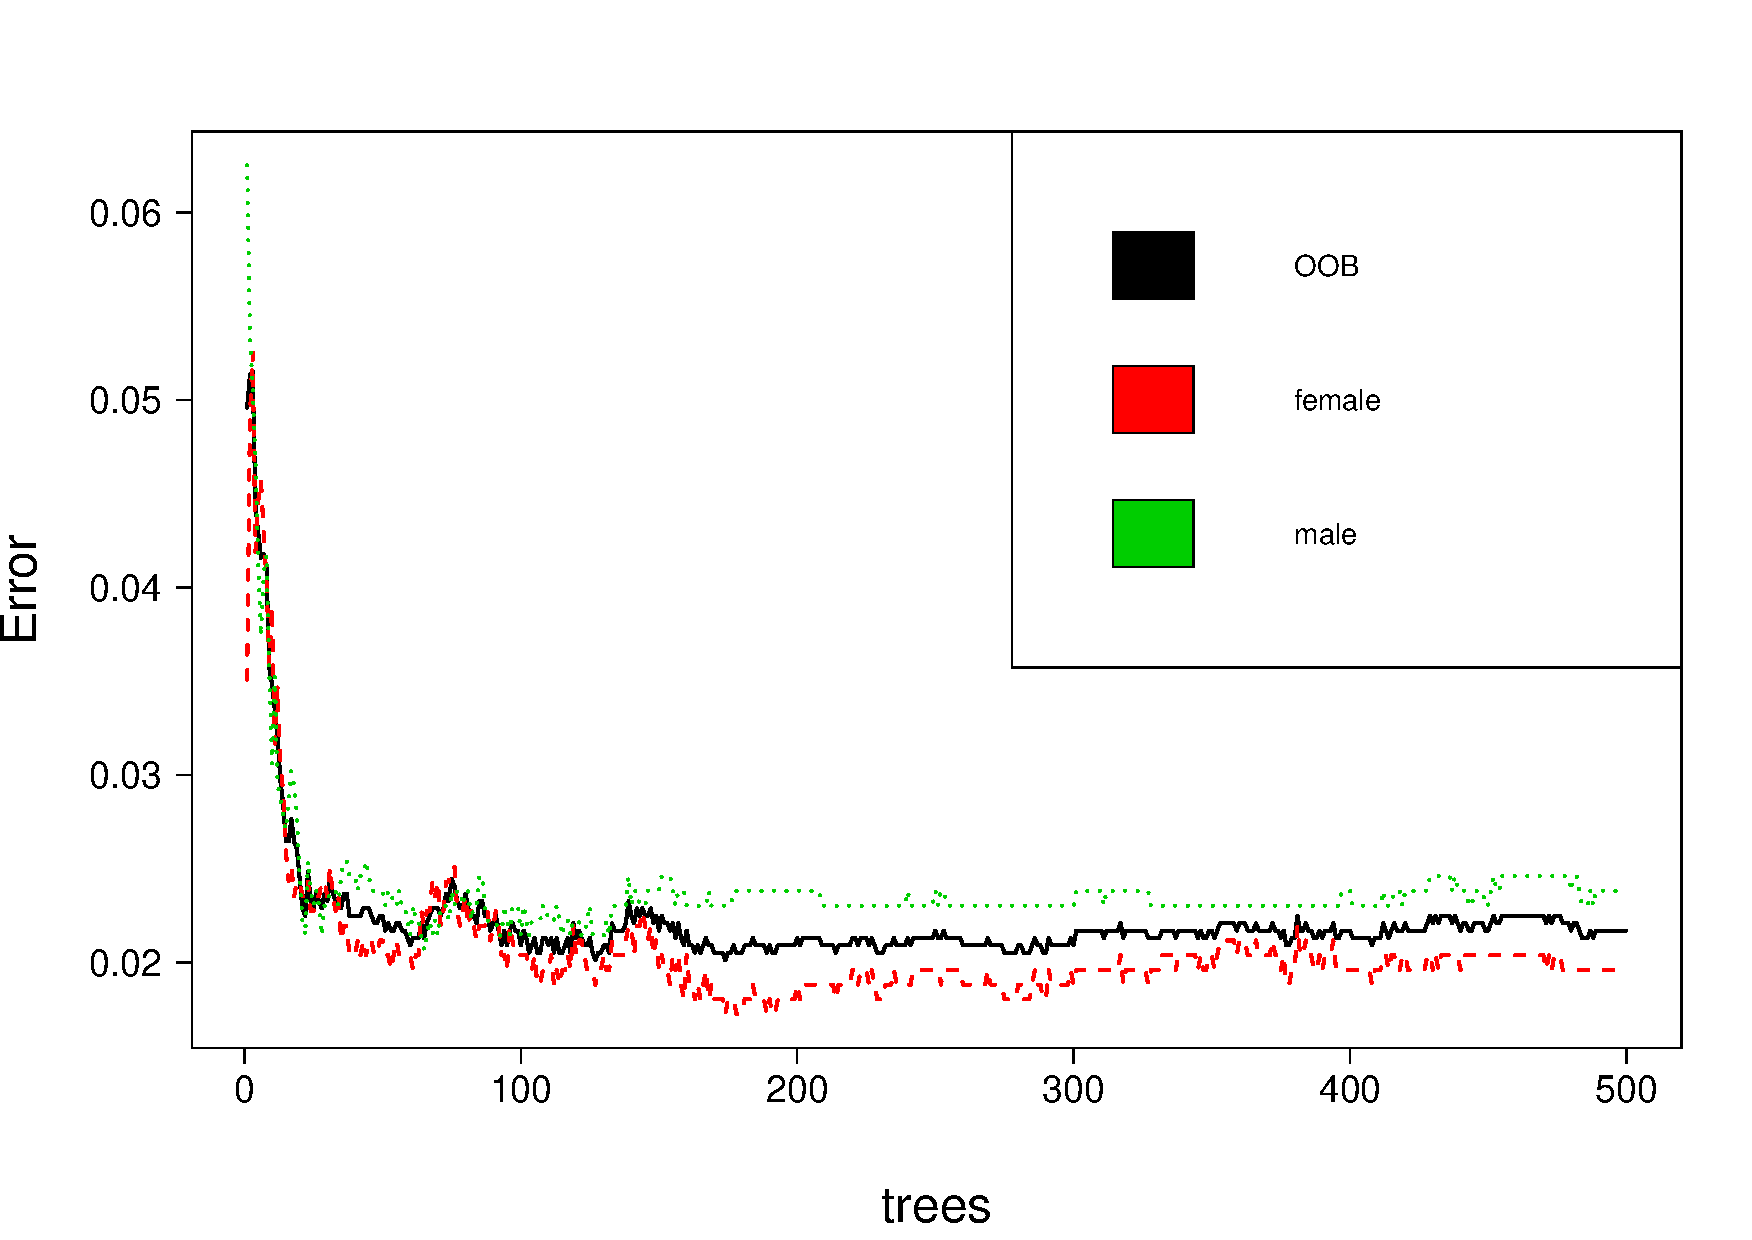
\includegraphics[height=\BoxPlotFigHeight]{figures/RF.pdf}}\hfill\null%
	\caption{Out-of-bag error estimate of (a)-bagging and (b)-random forest.}
	\label{fig_tree}
\end{figure}
%%%%%%%%%%%% END OF FIGURE %%%%%%%%%%%

Partial dependence plots are useful to interpret variable importance in complex ``black box'' methods, such as random forests. These plots illustrate the marginal effect of the selected feature after integrating out the other features. In Fig.~\ref{fig_partial_dep}, we present the partial dependence plot on ``meanfun''. The shape of the curve indicates that the fitted random forest uses a clear threshold that separate the two classes (female/male). Consequently, we can argue that the steepness of the curve in the middle pinpoints the importance of ``meanfun''. 
%%%%%%%%%%%% FIGURE %%%%%%%%%%%
\settoheight{\BoxPlotFigHeight}{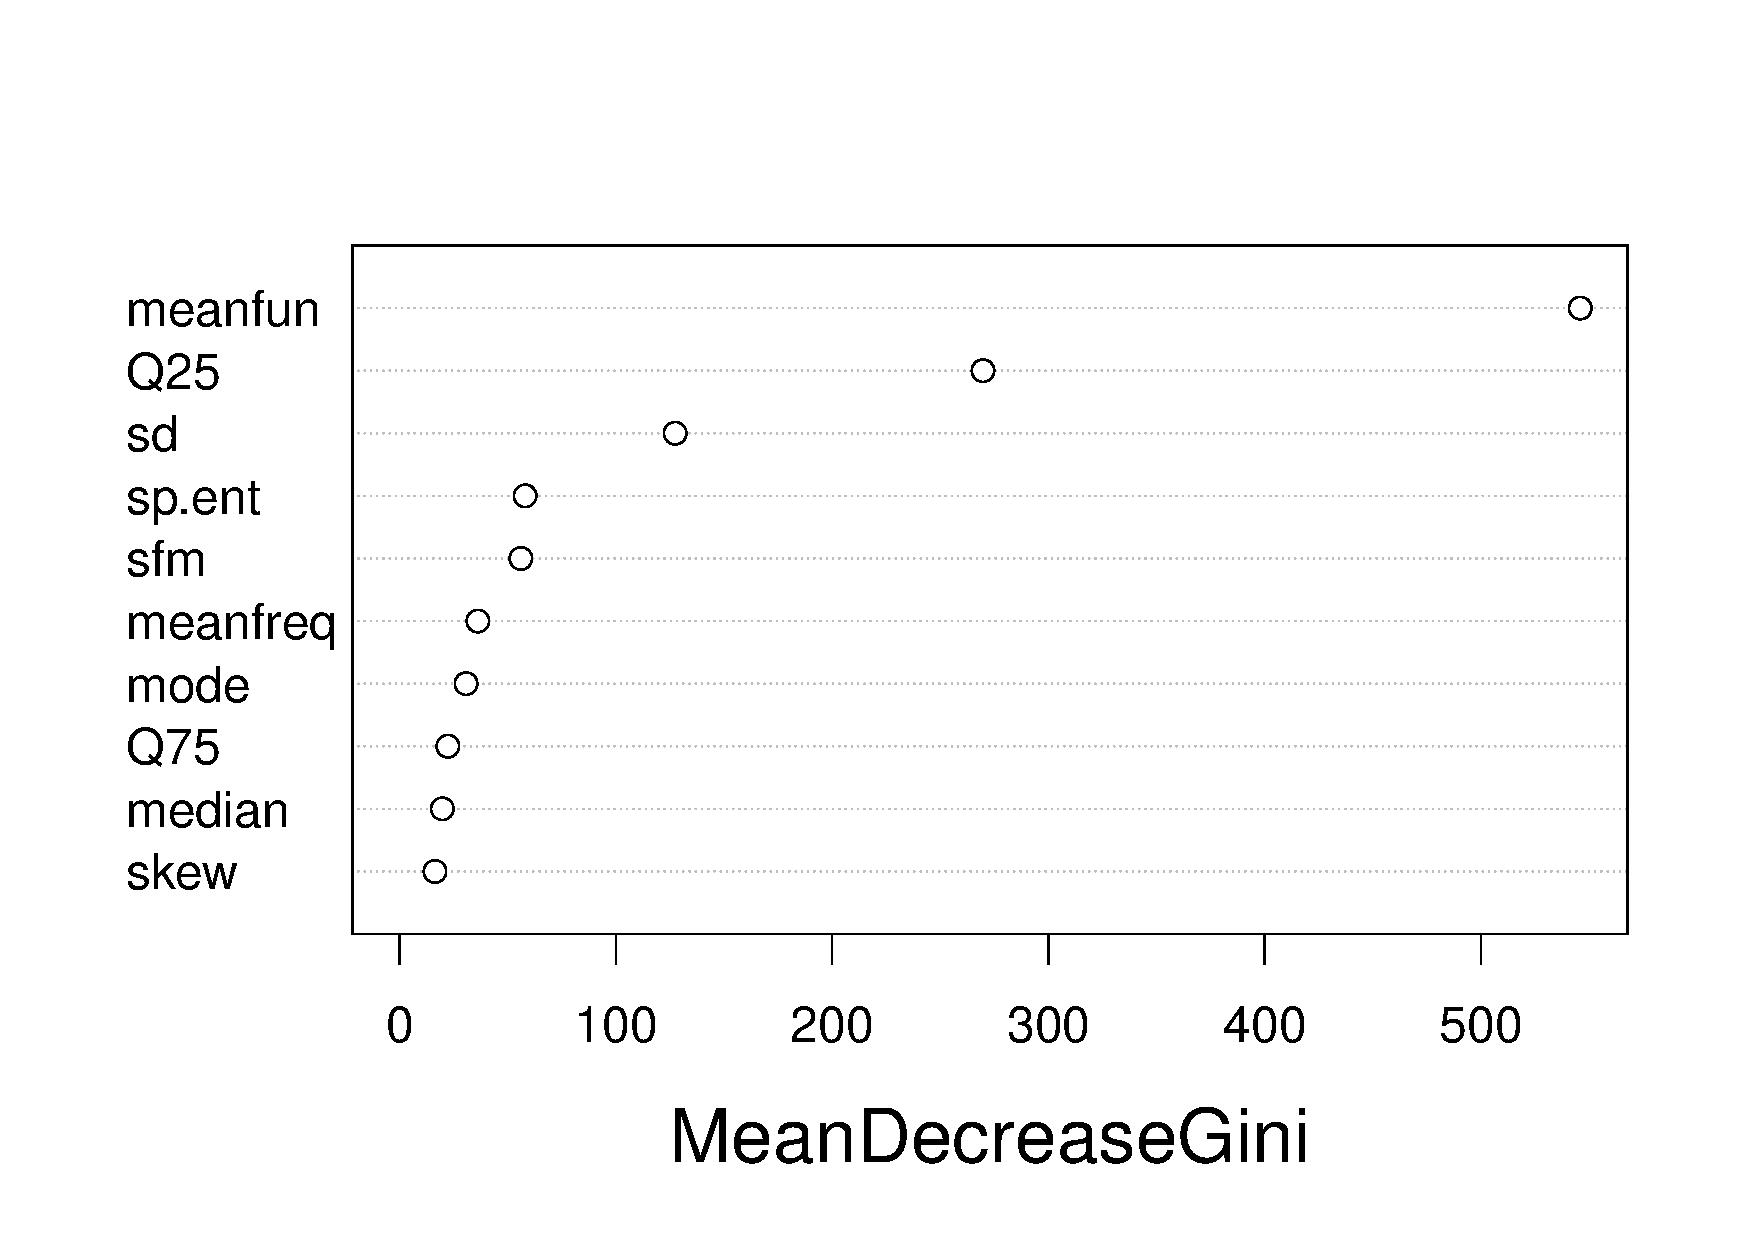
\includegraphics[width=\BoxPlotFigWidth]{figures/meanDecreaseGini.pdf}}
\begin{figure}[htb]
	% Maximum length
	\hfill%
	\subcaptionbox{\label{fig_partial_dep}}{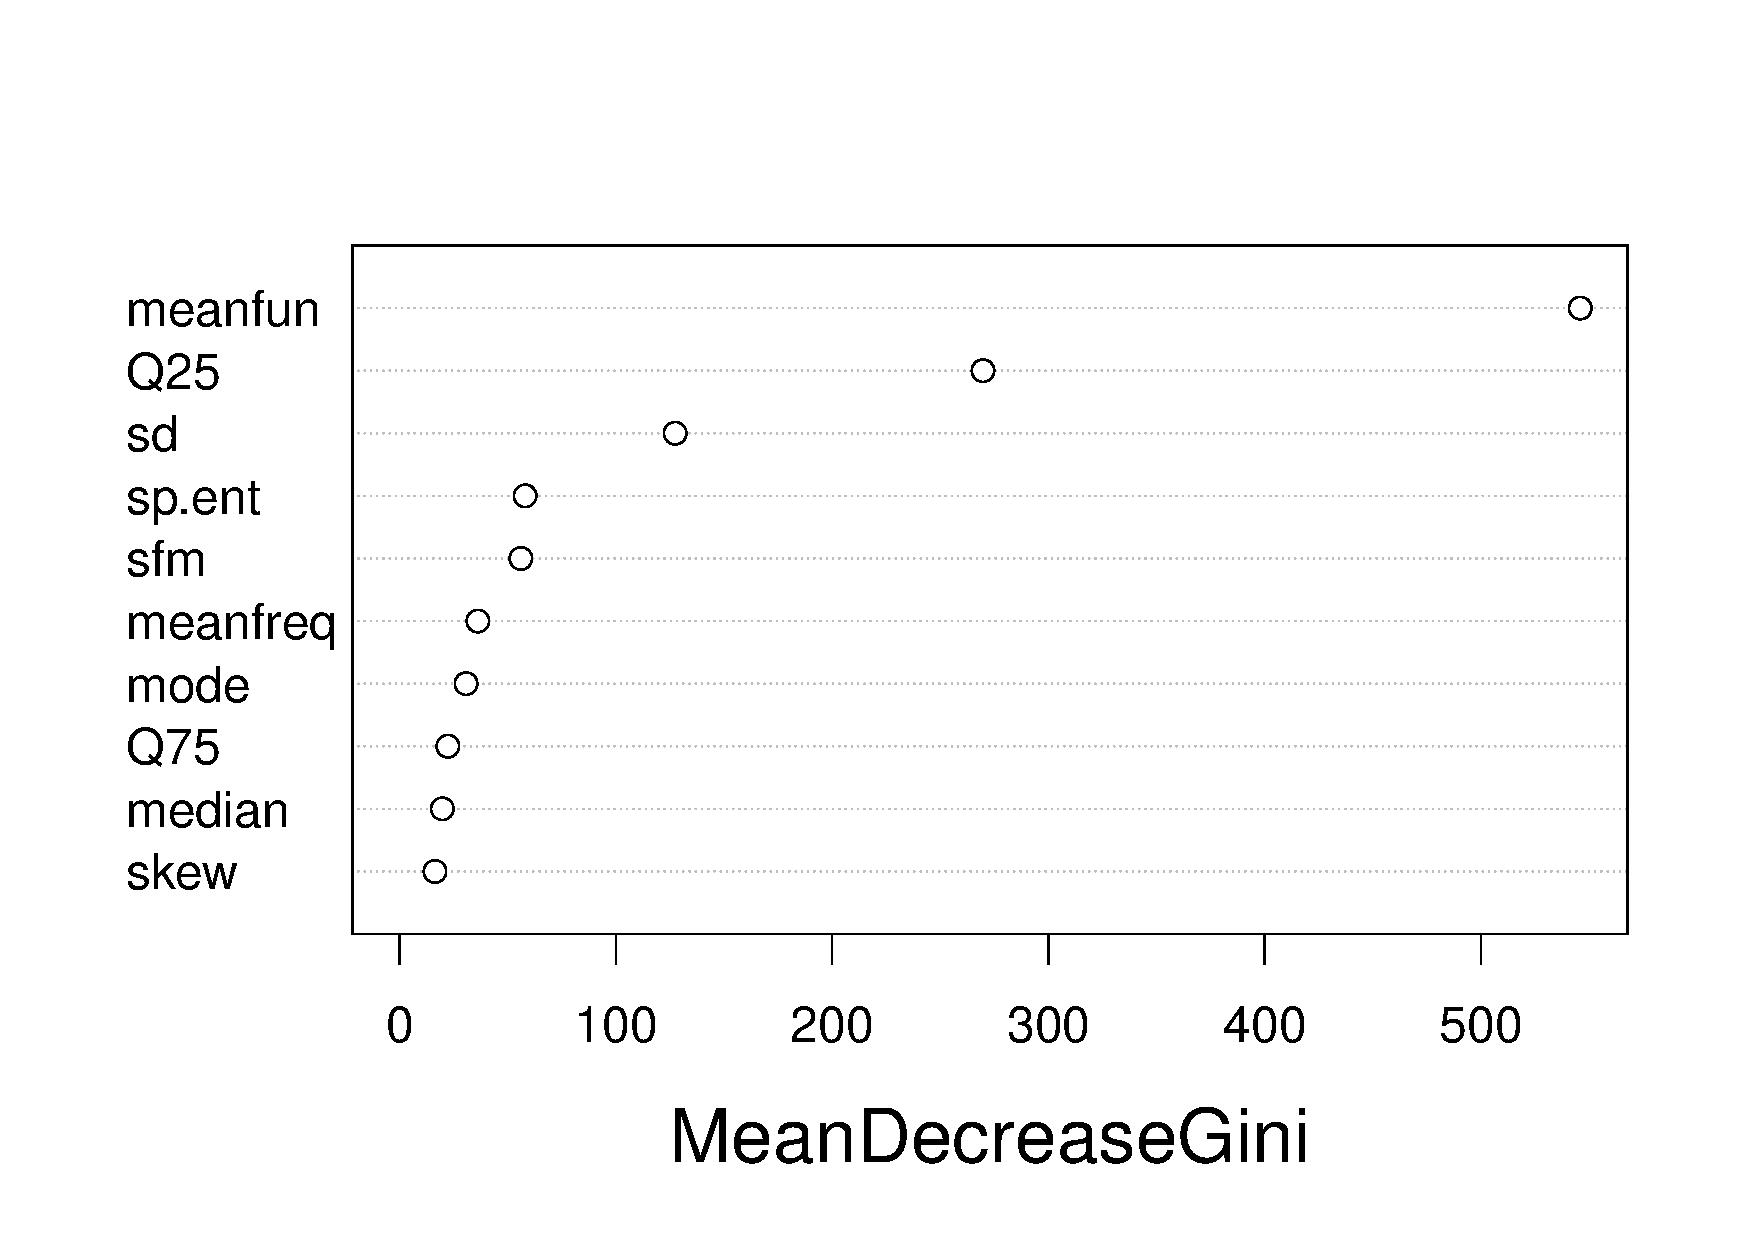
\includegraphics[height=\BoxPlotFigHeight]{figures/meanDecreaseGini.pdf}}\hfill%
	\subcaptionbox{\label{fig_feature_imp}}{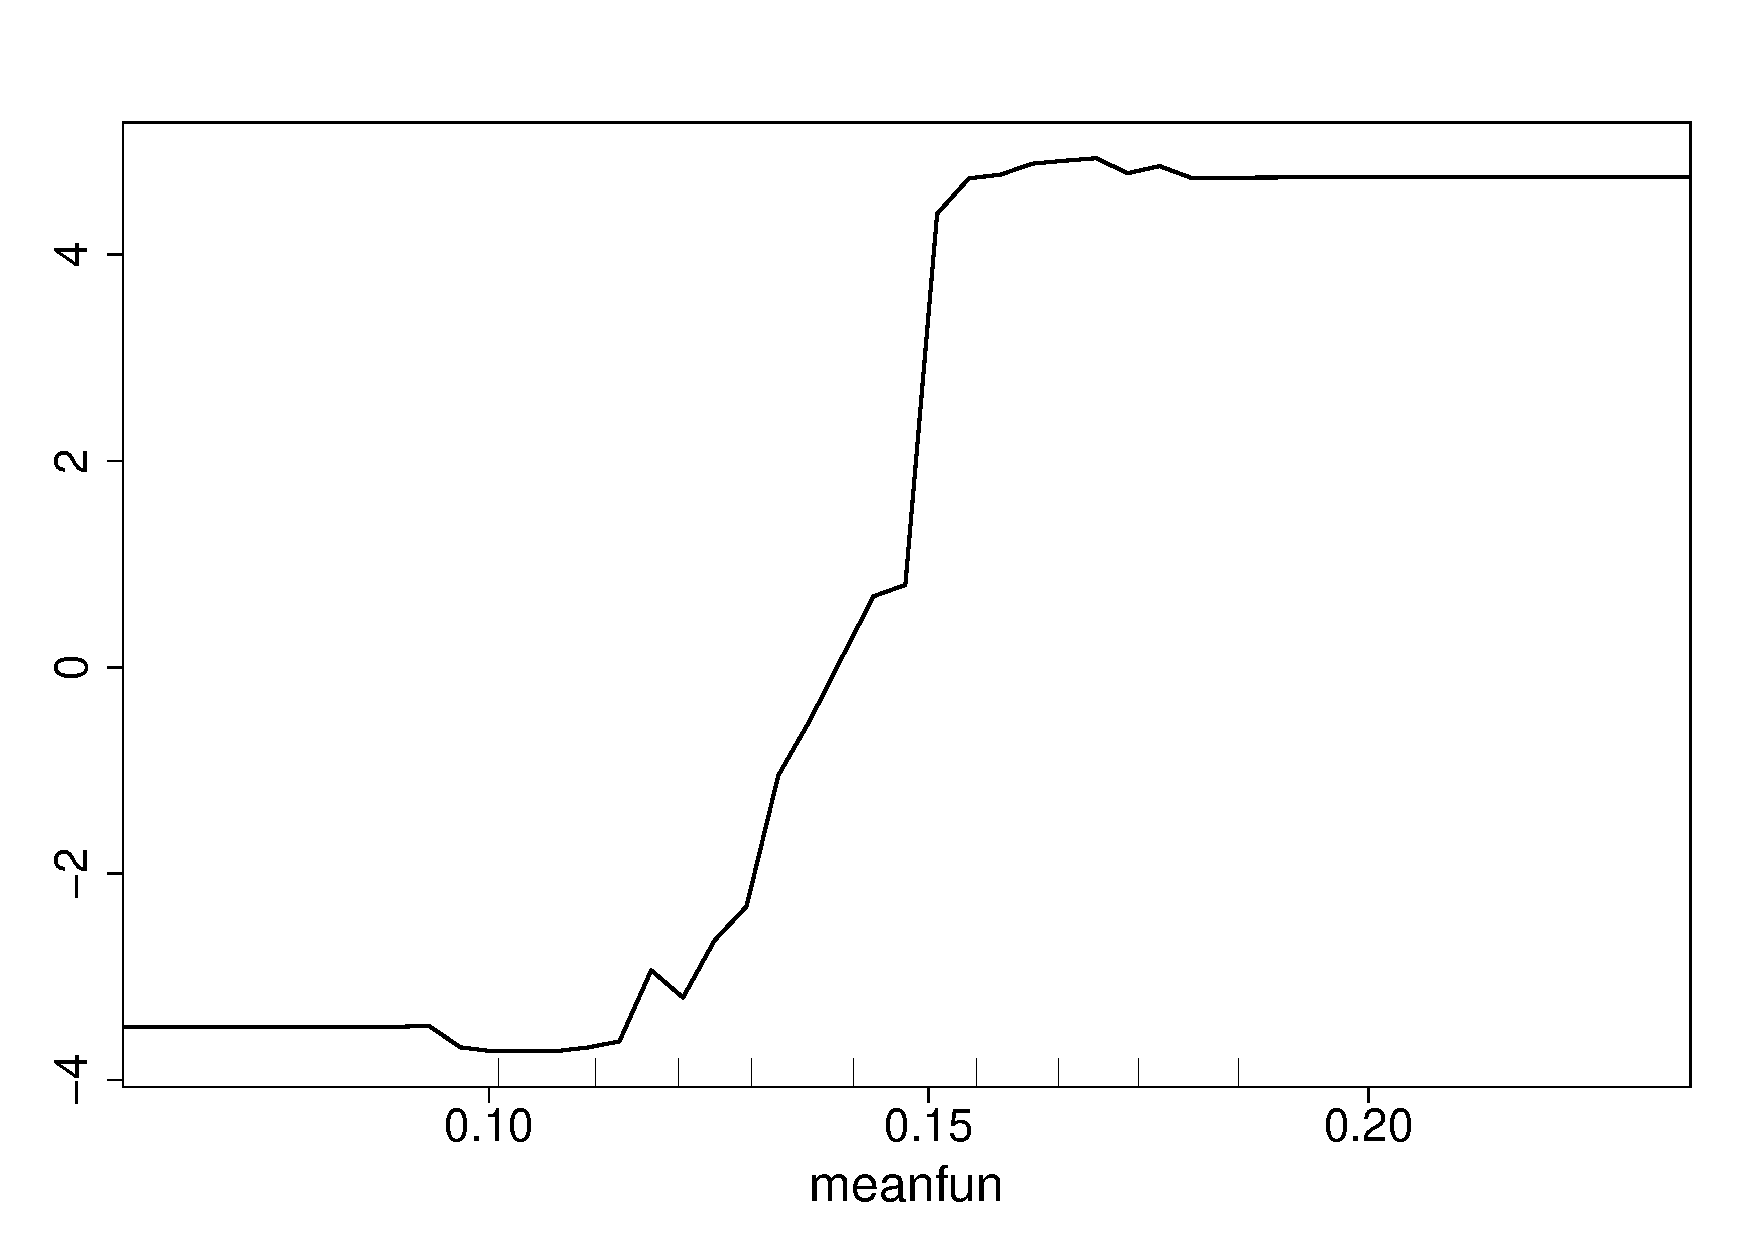
\includegraphics[height=\BoxPlotFigHeight]{figures/partialDependence.pdf}}\hfill\null%
	\caption{(a)-Feature importance based on the mean decrease of gini metric; (b)-Partial dependence with respect to the ``meanfun'' feature.}
	\label{fig_tree_feature}
\end{figure}
%%%%%%%%%%%% END OF FIGURE %%%%%%%%%%%
\paragraph{Gradient tree boosting}
In our quest of determining the model with the best accuracy, we then implement gradient tree boosting by using XGBoost R package\footnote{\url{https://cran.r-project.org/src/contrib/Archive/xgboost/}}. We choose stumps, which are simple trees with two leaves, to be the slow learners. We obtain a test error of \num{0.0189}, which confirms the superiority of boosting compared to trees and bagged trees.
\subsection{Support vector machines}
\paragraph{SVM with a linear kernel}
We apply SVM with a simple linear kernel using \num{10}-fold cross validation for parameter selection. We obtain a test error of \num{0.0142}.
\paragraph{SVM with a RBF kernel}
Finally, we implement SVM with a gaussian radial kernel. \num{10}-fold cross validation is used to determine the best combination of the kernel parameter $ \gamma $ and the margin parameter $C$. 
\subsection{Conclusion}
The analysis conducted above, using all available features, confirms that ``meanfun'' plays indeed an integral role in gender recognition by voice. Variable importance metrics of random forests highlight that ``meanfun'' is substantially more important than the rest of the features. Simultaneously, the results obtained from (Lasso) logistic regression, pinpoint the fact that some predictors are not significant and, thus, not useful in improving predictive performance.

Nevertheless, we observe that using all features instead of only ``meanfun'', decreases the test errors of discussed models. Since we are also interested in specifying the model with the lowest classification error, it makes sense to take into account all \num{17} variables. However, as Table~\ref{tab_res_naive} indicates, model performances seem to be highly dependent on the initial training/test error split. Therefore, we cannot draw a conclusion about the best classifier and we have to refine our approach of model assessment.
\section{Classification based on a $50/50$ split of the dataset}
\label{sec_our_strat}
\subsection{Experimental settings}
In order to decrease the variance, we suggest to use another strategy described hereafter. 
First we perform a $50/50$ split of the dataset and we obtain two subsets of same dimension, denoted as $S1$ and $S2$.
We use $S1$ to perform best parameter selection based on \num{10}-fold cross validation.
We use $S2$ for model comparison based on averaging of the classification error estimates on \num{5} folds, where the classification error estimate is computed as the $0-1$ loss. 
The advantage of such an approach is that the averaging induced by the \num{5} folds should reduce the variance, while keeping a relatively low bias because of the size of $S2$. 

As in Section~\ref{sec_naive_strat}, the errors are computed for \num{5} seed numbers in order to study the variability of the models and the results are reported in Table~\ref{tab_res_our_strategy}.

\begin{table}[htb]
	\ra{1.2}
	\caption{Classification Error Estimate of the Methods for Different Seed Numbers With $50/50$ Split}
	\begin{center}
		\begin{tabular}{@{} c c c  c c c c c c@{}}\toprule
			\multirow{2}{*}{Type} & \multirow{2}{*}{Methods} &  \multicolumn{5}{c}{Seed number}
			& 	\multirow{2}{*}{Mean} & \multirow{2}{*}{Std.} \\
			& & 1 & 2 & 3 & 4 & 5 & & \\
			\midrule
			\multirow{5}{*}{Max. Lik.} & Log. reg. & \num{0.0221} & \num{0.0262} & \num{0.0310} & \num{0.0261} & \num{0.0291} & \num{0.0269} & \num{0.00339} \\
			& Log. reg. - $\ell_2$ & \num{0.0196} & \num{0.0214} & \num{0.0305} & \num{0.0248} & \num{0.0278} & \num{0.0248} & \num{0.00449}\\
			& Log. reg. - $\ell_1$ & \num{0.0284} & \num{0.0294} & \num{0.0368} & \num{0.0348} & \num{0.0364} & \num{0.0332} & \num{0.00397}\\
			& LDA & \num{0.0291} & \num{0.0269} & \num{0.0342} & \num{0.0309} & \num{0.0313} & \num{0.0305} & \num{0.00274}\\
			& QDA & \num{0.0280} & \num{0.0257} & \num{0.0370} & \num{0.0362} & \num{0.0365} & \num{0.0327} & \num{0.00542}\\
			\cmidrule{1-9}
			\multirow{5}{*}{Trees} & Tree & \num{0.0284} & \num{0.0317} & \num{0.0387} & \num{0.0454} & \num{0.0468} & \num{0.0382} & \num{0.00814}\\
			& Pruned Tree & \num{0.0229} & \num{0.0296} & \num{0.0356} & \num{0.0454} & \num{0.0567} & \num{0.0355} & \num{0.0133}\\  
			& Bagging & \num{0.0209} & \num{0.0244} & \num{0.0319} & \num{0.0253} & \num{0.0302} & \num{0.0266} & \num{0.00445}\\
			& Random Forest & \num{0.0191} & \num{0.0206} & \num{0.0305} & \num{0.0248} & \num{0.0290} & \num{0.0248} & \num{0.00500}\\
			& XGBoost & \textbf{\num{0.0170}} & \textbf{\num{0.0149}} & \textbf{\num{0.0259}} & \textbf{\num{0.0197}} & \textbf{\num{0.0227}} & \textbf{\num{0.0201}} & \num{0.00439}\\
			\cmidrule{1-9}
			\multirow{2}{*}{SVM} & Linear & \num{0.0209} & \num{0.0269} & \num{0.0286} & \num{0.0229} & \num{0.0291} & \num{0.0249} & \num{0.00362}\\
			& Gaussian & \num{0.0184} & \num{0.0188} & \num{0.0272} & \num{0.0211} & \num{0.0234} & \num{0.0218} & \num{0.00361}\\
			\cmidrule{1-9}
			x & kNN & \num{0.0273} & \num{0.0312} & \num{0.0326} & \num{0.0410} & \num{0.0382} & \num{0.0340} & \num{0.00551} \\
			\bottomrule
		\end{tabular}
	\end{center}
	\label{tab_res_our_strategy}
\end{table}
\subsection{Results and best classification method}
From Table~\ref{tab_res_our_strategy}, it can be noticed that the proposed strategy:
\begin{itemize}
	\item gives very similar results to the $80/20$ split regarding the classification error estimates of the different methods;
 	\item tends to decrease the variance of the error estimate with respect to the seed number. Indeed, the average standard deviation of the error estimate over the different estimators is \num{0.00523} while it was \num{0.00636} with the $80/20$ split.
\end{itemize} 
Surprisingly, the variance reduction does not work for all the methods. For instance, QDA has a higher variance with the proposed strategy than with the $80/20$ split. 
This can be explained by the fact that a \num{5}-fold cross validation is not sufficient to significantly reduce the variance. However, we believe that, given the amount of data, increasing the number of folds may have a significant impact on the bias. 

Nevertheless, the proposed strategy allows us to identify that XGBoost slightly outperforms other tree-based methods as well as the SVM with the RBF kernel. It is therefore chosen as the best classification model for our gender classification task. 
%%%%%%%%%%%% FIGURE %%%%%%%%%%%
\settoheight{\BoxPlotFigHeight}{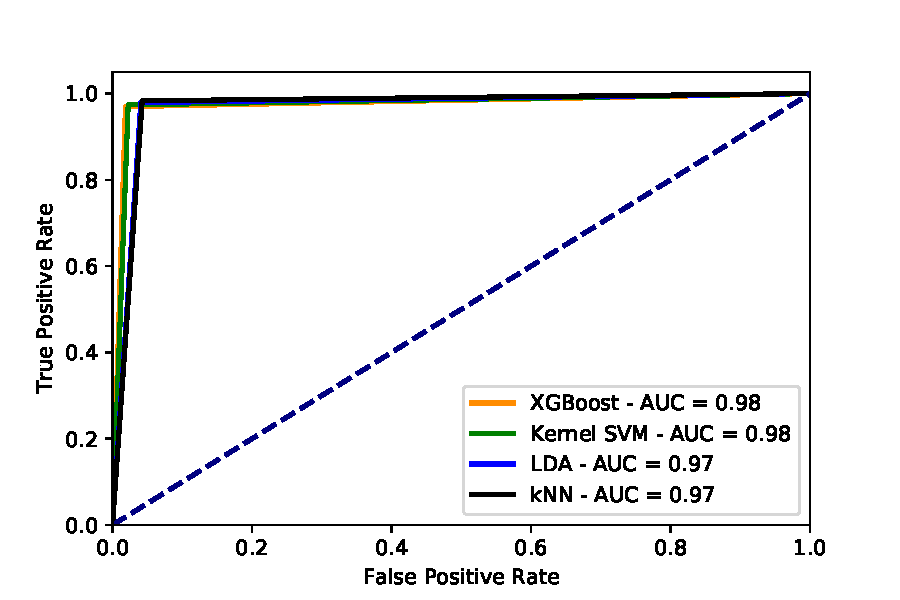
\includegraphics[width=\BoxPlotFigWidth]{figures/ROC_generic.pdf}}
\begin{figure}[htb]
	% Maximum length
	\hfill%
	\subcaptionbox{\label{fig_roc_generic}}{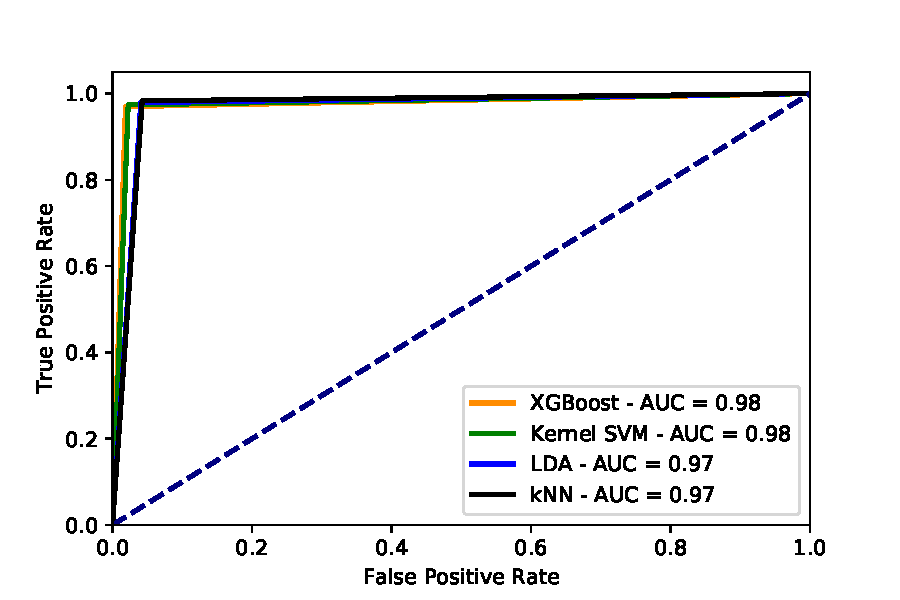
\includegraphics[height=\BoxPlotFigHeight]{figures/ROC_generic.pdf}}\hfill%
	\subcaptionbox{\label{fig_roc_zoomed}}{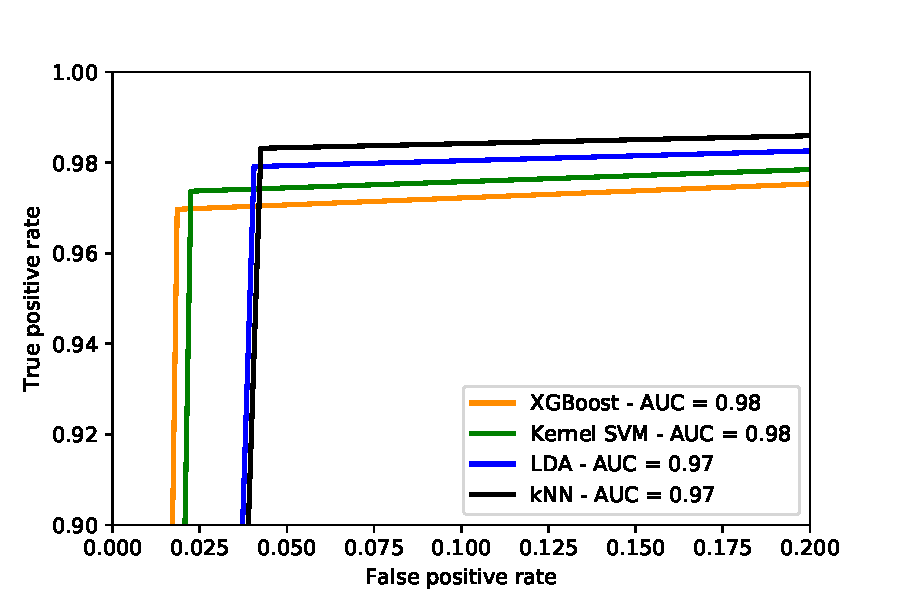
\includegraphics[height=\BoxPlotFigHeight]{figures/ROC_zoom.pdf}}\hfill\null%
	\caption{(a)-ROC curves for XGBoost~(orange), Kernel SVM~(green), LDA~(blue) and kNN~(black); (b)-ROC curves in a region around the transition.}
	\label{fig_tree_feature}
\end{figure}
%%%%%%%%%%%% END OF FIGURE %%%%%%%%%%%

The receiver operating characteristics~(ROC) curves of XGBoost, Kernel SVM, LDA and kNN ,displayed on Fig.~\ref{fig_roc_generic}, highlight the fact that the different classification methods are close. A finer analysis at the transition, displayed on Fig.~\ref{fig_roc_zoomed}, shows that the superiority of XGBoost does not come from a higher true positive rate than the other methods, but from its ability to reach high true positive rates for for lower false positive rates than the other methods.  